% lecture3_ro.tex -- GENERATED by build_L3.py from L3_numbers.json; do not edit by hand.
\documentclass[10pt,aspectratio=169,t]{beamer}
% =============================================================================
% nn_preamble.tex -- shared Beamer preamble of Neural Networks and Deep Learning (NN)
% Used by every lecture: lectures/Lk/lecturek.tex does
%   \documentclass[10pt,aspectratio=169,t]{beamer}
%   % =============================================================================
% nn_preamble.tex -- shared Beamer preamble of Neural Networks and Deep Learning (NN)
% Used by every lecture: lectures/Lk/lecturek.tex does
%   \documentclass[10pt,aspectratio=169,t]{beamer}
%   % =============================================================================
% nn_preamble.tex -- shared Beamer preamble of Neural Networks and Deep Learning (NN)
% Used by every lecture: lectures/Lk/lecturek.tex does
%   \documentclass[10pt,aspectratio=169,t]{beamer}
%   \input{../common/nn_preamble}
%   \nnlecture{k}{Lecture title}
% Logos live in lectures/common/logos/, charts in lectures/Lk/charts/.
% Do NOT add \hfuzz / \vfuzz / \hbadness here: overfull boxes must be fixed, not hidden.
% =============================================================================

\usetheme{default}
\setbeamersize{text margin left=7mm, text margin right=7mm}

% ---------------------------------------------------------------- packages
\usepackage[utf8]{inputenc}
\usepackage[T1]{fontenc}
\usepackage{lmodern}
\usepackage{amsmath, amssymb}
\usepackage{mathtools}
\usepackage{bm}
\usepackage{tikz}
\usetikzlibrary{arrows.meta, positioning, calc, shapes.misc}
\usepackage{booktabs}
\usepackage{array}
\usepackage{graphicx}
\usepackage{colortbl}
\usepackage{xcolor}
\usepackage{multicol}
\hypersetup{colorlinks=true, linkcolor=MainBlue, urlcolor=MainBlue, citecolor=MainBlue}
\graphicspath{{../common/logos/}}   % charts are included with their language folder: charts/en/, charts/ro/

% ---------------------------------------------------------------- colours
\definecolor{MainBlue}{RGB}{26, 58, 110}
\definecolor{IDAred}{RGB}{205, 0, 0}
\definecolor{DarkGray}{RGB}{51, 51, 51}
\definecolor{FooterGray}{RGB}{100, 100, 100}
\definecolor{BlockGray}{RGB}{236, 238, 242}
\definecolor{KeynoteGray}{RGB}{218, 218, 218}
\definecolor{Crimson}{RGB}{190, 40, 50}
\definecolor{Forest}{RGB}{30, 110, 50}
\definecolor{Bitter}{RGB}{214, 150, 20}
% chart palette (same hex values and order as lectures/common/nn_plot.py SERIES)
\definecolor{Ser1}{HTML}{2A78D6}
\definecolor{Ser2}{HTML}{EB6834}
\definecolor{Ser3}{HTML}{1BAF7A}
\definecolor{Ser4}{HTML}{EDA100}
\definecolor{Ser5}{HTML}{E87BA4}
\definecolor{Ser6}{HTML}{008300}
\definecolor{Ser7}{HTML}{6250D6}
\definecolor{Ser8}{HTML}{E34948}

\setbeamertemplate{background}{%
  \begin{tikzpicture}[remember picture, overlay]
    \shade[shading=axis, shading angle=315, top color=white, bottom color=KeynoteGray]
      (current page.south west) rectangle (current page.north east);
  \end{tikzpicture}}
\setbeamercolor{background canvas}{bg=}
\setbeamercolor{structure}{fg=MainBlue}
\setbeamercolor{normal text}{fg=DarkGray}
\setbeamercolor{title}{fg=IDAred}
\setbeamercolor{frametitle}{fg=IDAred, bg=}
\setbeamercolor{block title}{bg=MainBlue, fg=white}
\setbeamercolor{block body}{bg=BlockGray, fg=DarkGray}
\setbeamercolor{block title alerted}{bg=Crimson, fg=white}
\setbeamercolor{block body alerted}{bg=Crimson!7, fg=DarkGray}
\setbeamercolor{block title example}{bg=Forest, fg=white}
\setbeamercolor{block body example}{bg=Forest!7, fg=DarkGray}
\setbeamercolor{item}{fg=MainBlue}
\setbeamerfont{frametitle}{size=\large, series=\bfseries}
\setbeamerfont{block title}{size=\small, series=\bfseries}
\setbeamertemplate{blocks}[rounded][shadow=false]
\setbeamertemplate{itemize item}{\color{MainBlue}$\boxdot$}
\setbeamertemplate{itemize subitem}{\color{MainBlue}\scriptsize$\blacktriangleright$}
% compact two-level lists: level 1 = main point, level 2 = details (no text outside bullets)
\setbeamerfont{itemize/enumerate subbody}{size=\footnotesize}
\setlength{\leftmargini}{1.1em}
\setlength{\leftmarginii}{1.1em}
\setbeamertemplate{itemize/enumerate body begin}{\setlength{\topsep}{0pt}\setlength{\partopsep}{0pt}\setlength{\parskip}{0pt}}
\setbeamertemplate{itemize/enumerate subbody begin}{\setlength{\topsep}{0pt}\setlength{\partopsep}{0pt}\setlength{\itemsep}{0pt}\vspace{-0.4ex}}

\setbeamertemplate{enumerate item}{\color{MainBlue}\insertenumlabel.}
\setlength{\leftmargini}{1.3em}
\setlength{\leftmarginii}{1.2em}
\setbeamertemplate{navigation symbols}{}
\setbeamertemplate{section in toc}{\color{MainBlue}$\blacktriangleright$~\inserttocsection}
\setbeamertemplate{caption}{\raggedright\insertcaption\par}
% frame subtitle = precise citation line under the claim title (Weron style)
\setbeamerfont{framesubtitle}{size=\footnotesize}
\setbeamercolor{framesubtitle}{fg=FooterGray}
% outline that reappears at every section with the current section highlighted
\setbeamertemplate{section in toc shaded}[default][35]
\setbeamertemplate{subsection in toc shaded}[default][35]
\setbeamertemplate{subsection in toc}{\leavevmode\leftskip=2.2em\color{DarkGray}\small\inserttocsubsection\par}
\AtBeginSection[]{{\begin{frame}{\txtoutline}\vspace{2mm}\small
  \tableofcontents[currentsection,hideothersubsections]\end{frame}}}

% ---------------------------------------------------------------- head and foot
\setbeamertemplate{headline}{%
  \vskip10pt%
  \hbox to \paperwidth{\hskip0.5cm%
    {\small\color{FooterGray}\renewcommand{\hyperlink}[2]{##2}\insertsectionhead}%
    \hfill\textcolor{FooterGray}{\small\insertframenumber}\hskip0.5cm}%
  \vskip4pt{\color{FooterGray}\hrule height 0.4pt}}
% footer as in the other courses (MFM, SFM): course name on the left, small sparkline on the right
\setbeamertemplate{footline}{%
  {\color{FooterGray}\hrule height 0.4pt}\vskip4pt%
  \hbox to \paperwidth{\hskip0.5cm%
    \textcolor{FooterGray}{\small\txtcourse}%
    \hfill\raisebox{-0.1em}{\begin{tikzpicture}[x=0.08em, y=0.08em, line width=0.4pt]
      \draw[FooterGray] (0,3) -- (1,4) -- (2,3.5) -- (3,5) -- (4,4) -- (5,6) -- (6,5.5) -- (7,4) -- (8,5) -- (9,7) -- (10,6) -- (11,5) -- (12,6.5) -- (13,8) -- (14,7) -- (15,6) -- (16,7.5) -- (17,9) -- (18,8) -- (19,7) -- (20,8.5) -- (21,10) -- (22,9) -- (23,8) -- (24,9.5);
    \end{tikzpicture}}\hskip0.5cm}%
  \vskip6pt}

% ---------------------------------------------------------------- title page
\defbeamertemplate*{title page}{nn}[1][]{%
  \vspace{0.15cm}
  \begin{center}
    \href{https://www.ase.ro}{
\includegraphics[height=0.9cm]{ase_logo.png}}\hspace{0.3cm}%
    \href{https://ipe.ro/new}{
\includegraphics[height=0.9cm]{acad_logo.png}}\hspace{0.3cm}%
    \href{https://theida.net}{
\includegraphics[height=0.9cm]{ida_logo.png}}\hspace{0.3cm}%
    \href{https://blockchain-research-center.com}{
\includegraphics[height=0.9cm]{brc_logo.png}}\hspace{0.3cm}%
    \href{https://www.ai4efin.ase.ro}{
\includegraphics[height=0.9cm]{ai4efin_logo.png}}\hspace{0.3cm}%
    \href{https://www.digital-finance-msca.com}{
\includegraphics[height=0.9cm]{msca_logo.png}}%
  \end{center}
  \vspace{0.45cm}
  \begin{center}
    \begin{minipage}{0.1\textwidth}\centering
      \href{https://quantlet.com}{
\includegraphics[height=0.9cm]{ql_logo.png}}\end{minipage}%
    \begin{minipage}{0.78\textwidth}\centering
      {\Large\bfseries\usebeamercolor[fg]{title}\inserttitle}\par\vspace{0.25cm}
      {\large\usebeamercolor[fg]{title}\insertsubtitle}\end{minipage}%
    \begin{minipage}{0.1\textwidth}\centering
      \href{https://quantinar.com}{
\includegraphics[height=0.9cm]{qr_logo.png}}\end{minipage}
  \end{center}
  \vfill
  \hspace{0.4cm}{\bfseries\insertauthor}\par\vspace{0.12cm}
  \hspace{0.4cm}\begin{minipage}[t]{0.92\textwidth}\raggedright\footnotesize\insertinstitute\end{minipage}
  \par\vspace{0.4cm}}

% ---------------------------------------------------------------- lecture metadata
\newcommand{\nnshort}{}
\newcommand{\nnnb}{notebooks}
\newcommand{\nnrepo}{https://github.com/danpele/NEURAL_BIZ/tree/main}
% language-dependent labels (English default; \nnromanian switches to Romanian, call it before \nnlecture)
\newcommand{\txtcourse}{Neural Networks and Deep Learning}
\newcommand{\txtlecture}{Lecture}
\newcommand{\txtoutline}{Outline}
\newcommand{\txtintuition}{In one sentence:}
\newcommand{\txtjob}{In practice:}
\newcommand{\txttry}{Experiment yourself:}
\newcommand{\txtwhere}{where}
\newcommand{\txtsim}{SIMULATED DATA (teaching illustration)}
\newcommand{\txtnbsuffix}{}
\newcommand{\txtinstitute}{Bucharest University of Economic Studies (ASE), Department of Statistics and Econometrics\\
    Romanian Academy, Institute for Economic Forecasting (IPE)\\
    IDA Institute Digital Assets \textbullet\ AI4EFin \textbullet\ MSCA Digital Finance}
\newcommand{\nnromanian}{%
  \renewcommand{\txtcourse}{Rețele neuronale și deep learning}%
  \renewcommand{\txtlecture}{Cursul}%
  \renewcommand{\txtoutline}{Cuprins}%
  \renewcommand{\txtintuition}{Pe scurt:}%
  \renewcommand{\txtjob}{În practică:}%
  \renewcommand{\txttry}{Exercițiu practic:}%
  \renewcommand{\txtwhere}{unde}%
  \renewcommand{\txtsim}{DATE SIMULATE (doar pentru ilustrare)}%
  \renewcommand{\txtnbsuffix}{\string_ro}%
  \renewcommand{\txtinstitute}{Academia de Studii Economice din București (ASE), Departamentul de Statistică și Econometrie\\
    Academia Română, Institutul de Prognoză Economică (IPE)\\
    IDA Institute Digital Assets \textbullet\ AI4EFin \textbullet\ MSCA Digital Finance}}
\newcommand{\nnlecture}[2]{%
  \renewcommand{\nnshort}{\txtlecture\ #1}%
  \renewcommand{\nnnb}{notebooks/L#1\string_notebook\txtnbsuffix.ipynb}%
  \title[NN]{\txtcourse}%
  \subtitle{\txtlecture\ #1: #2}%
  \author{Prof.\ dr.\ Daniel Traian PELE}%
  \institute{\txtinstitute}%
  \date{}}

% ---------------------------------------------------------------- teaching blocks (one message per frame)
% \intuition{one plain sentence}  ->  formula with every symbol defined  ->  real-data example  ->  \manager{one line}
\newcommand{\intuition}[1]{\begin{itemize}\item {\color{MainBlue}\textbf{\txtintuition}}~#1\end{itemize}\vspace{0.6mm}}
\newcommand{\manager}[1]{\colorbox{Forest!10}{\parbox{\dimexpr\linewidth-2\fboxsep\relax}{\footnotesize
  \begin{itemize}\setlength{\itemsep}{0pt}\item \textbf{\color{Forest}\txtjob}~#1\end{itemize}}}}
% Experiment yourself: pointer to the matching notebook section
\newcommand{\tryit}[1]{{\scriptsize\href{\nnrepo/\nnnb}{%
  \raisebox{-0.15em}{
\includegraphics[height=0.85em]{ql_logo.png}}\,\textbf{\txttry}~\color{MainBlue}#1}}}
% bottom row: manager line (left) + experiment pointer (right), pinned to the bottom of the frame
\newcommand{\bottomrow}[2]{\par\vfill\noindent\begin{minipage}[b]{0.72\linewidth}#1\end{minipage}\hfill
  \begin{minipage}[b]{0.26\linewidth}\raggedleft #2\end{minipage}\par\vspace{0.5mm}}
\newcommand{\where}[1]{{\footnotesize\textbf{\txtwhere}~#1\par}}

% ---------------------------------------------------------------- helpers
% chart source line under a figure: \chartsource{Source ...; period ...}
\newcommand{\chartsource}[1]{\par\vspace{1pt}{\scriptsize\color{FooterGray}#1\par}}
% link to code: \quantlet{label}{path inside the repo}
\newcommand{\quantlet}[2]{\par\vspace{1pt}\hfill\href{\nnrepo/#2}{%
  \raisebox{-0.15em}{
\includegraphics[height=0.75em]{ql_logo.png}}\textcolor{MainBlue}{\scriptsize\ #1}}}
% inline Quantlet link for the bottom-right corner of a frame: \qlink{label}{path inside the repo}
\newcommand{\qlink}[2]{{\scriptsize\href{\nnrepo/#2}{\raisebox{-0.15em}{
\includegraphics[height=0.85em]{ql_logo.png}}\,\textcolor{MainBlue}{#1}}}}
\newcommand{\simlabel}{\colorbox{Crimson!12}{\scriptsize\bfseries\color{Crimson}\txtsim}}
\newcommand{\E}{\mathbb{E}}
\newcommand{\Var}{\operatorname{Var}}
\newcommand{\Cov}{\operatorname{Cov}}
\newcommand{\Corr}{\operatorname{Corr}}
\newcommand{\asinh}{\operatorname{asinh}}
\newcommand{\iid}{\overset{\text{i.i.d.}}{\sim}}
\newcommand{\EUR}{EUR}
% deep-learning notation (Bishop & Bishop, 2024): vectors bold lower case, matrices bold upper case
\newcommand{\R}{\mathbb{R}}
\newcommand{\vx}{\mathbf{x}}
\newcommand{\vy}{\mathbf{y}}
\newcommand{\vz}{\mathbf{z}}
\newcommand{\vh}{\mathbf{h}}
\newcommand{\vw}{\mathbf{w}}
\newcommand{\vb}{\mathbf{b}}
\newcommand{\mW}{\mathbf{W}}
\newcommand{\mX}{\mathbf{X}}
\newcommand{\btheta}{\boldsymbol{\theta}}
\newcommand{\loss}{\mathcal{L}}
\newcommand{\dataset}{\mathcal{D}}
\DeclareMathOperator*{\argmin}{arg\,min}
\DeclareMathOperator*{\argmax}{arg\,max}
\DeclareMathOperator{\softmax}{softmax}
\DeclareMathOperator{\ReLU}{ReLU}
\DeclareMathOperator{\sigm}{\sigma}

%   \nnlecture{k}{Lecture title}
% Logos live in lectures/common/logos/, charts in lectures/Lk/charts/.
% Do NOT add \hfuzz / \vfuzz / \hbadness here: overfull boxes must be fixed, not hidden.
% =============================================================================

\usetheme{default}
\setbeamersize{text margin left=7mm, text margin right=7mm}

% ---------------------------------------------------------------- packages
\usepackage[utf8]{inputenc}
\usepackage[T1]{fontenc}
\usepackage{lmodern}
\usepackage{amsmath, amssymb}
\usepackage{mathtools}
\usepackage{bm}
\usepackage{tikz}
\usetikzlibrary{arrows.meta, positioning, calc, shapes.misc}
\usepackage{booktabs}
\usepackage{array}
\usepackage{graphicx}
\usepackage{colortbl}
\usepackage{xcolor}
\usepackage{multicol}
\hypersetup{colorlinks=true, linkcolor=MainBlue, urlcolor=MainBlue, citecolor=MainBlue}
\graphicspath{{../common/logos/}}   % charts are included with their language folder: charts/en/, charts/ro/

% ---------------------------------------------------------------- colours
\definecolor{MainBlue}{RGB}{26, 58, 110}
\definecolor{IDAred}{RGB}{205, 0, 0}
\definecolor{DarkGray}{RGB}{51, 51, 51}
\definecolor{FooterGray}{RGB}{100, 100, 100}
\definecolor{BlockGray}{RGB}{236, 238, 242}
\definecolor{KeynoteGray}{RGB}{218, 218, 218}
\definecolor{Crimson}{RGB}{190, 40, 50}
\definecolor{Forest}{RGB}{30, 110, 50}
\definecolor{Bitter}{RGB}{214, 150, 20}
% chart palette (same hex values and order as lectures/common/nn_plot.py SERIES)
\definecolor{Ser1}{HTML}{2A78D6}
\definecolor{Ser2}{HTML}{EB6834}
\definecolor{Ser3}{HTML}{1BAF7A}
\definecolor{Ser4}{HTML}{EDA100}
\definecolor{Ser5}{HTML}{E87BA4}
\definecolor{Ser6}{HTML}{008300}
\definecolor{Ser7}{HTML}{6250D6}
\definecolor{Ser8}{HTML}{E34948}

\setbeamertemplate{background}{%
  \begin{tikzpicture}[remember picture, overlay]
    \shade[shading=axis, shading angle=315, top color=white, bottom color=KeynoteGray]
      (current page.south west) rectangle (current page.north east);
  \end{tikzpicture}}
\setbeamercolor{background canvas}{bg=}
\setbeamercolor{structure}{fg=MainBlue}
\setbeamercolor{normal text}{fg=DarkGray}
\setbeamercolor{title}{fg=IDAred}
\setbeamercolor{frametitle}{fg=IDAred, bg=}
\setbeamercolor{block title}{bg=MainBlue, fg=white}
\setbeamercolor{block body}{bg=BlockGray, fg=DarkGray}
\setbeamercolor{block title alerted}{bg=Crimson, fg=white}
\setbeamercolor{block body alerted}{bg=Crimson!7, fg=DarkGray}
\setbeamercolor{block title example}{bg=Forest, fg=white}
\setbeamercolor{block body example}{bg=Forest!7, fg=DarkGray}
\setbeamercolor{item}{fg=MainBlue}
\setbeamerfont{frametitle}{size=\large, series=\bfseries}
\setbeamerfont{block title}{size=\small, series=\bfseries}
\setbeamertemplate{blocks}[rounded][shadow=false]
\setbeamertemplate{itemize item}{\color{MainBlue}$\boxdot$}
\setbeamertemplate{itemize subitem}{\color{MainBlue}\scriptsize$\blacktriangleright$}
% compact two-level lists: level 1 = main point, level 2 = details (no text outside bullets)
\setbeamerfont{itemize/enumerate subbody}{size=\footnotesize}
\setlength{\leftmargini}{1.1em}
\setlength{\leftmarginii}{1.1em}
\setbeamertemplate{itemize/enumerate body begin}{\setlength{\topsep}{0pt}\setlength{\partopsep}{0pt}\setlength{\parskip}{0pt}}
\setbeamertemplate{itemize/enumerate subbody begin}{\setlength{\topsep}{0pt}\setlength{\partopsep}{0pt}\setlength{\itemsep}{0pt}\vspace{-0.4ex}}

\setbeamertemplate{enumerate item}{\color{MainBlue}\insertenumlabel.}
\setlength{\leftmargini}{1.3em}
\setlength{\leftmarginii}{1.2em}
\setbeamertemplate{navigation symbols}{}
\setbeamertemplate{section in toc}{\color{MainBlue}$\blacktriangleright$~\inserttocsection}
\setbeamertemplate{caption}{\raggedright\insertcaption\par}
% frame subtitle = precise citation line under the claim title (Weron style)
\setbeamerfont{framesubtitle}{size=\footnotesize}
\setbeamercolor{framesubtitle}{fg=FooterGray}
% outline that reappears at every section with the current section highlighted
\setbeamertemplate{section in toc shaded}[default][35]
\setbeamertemplate{subsection in toc shaded}[default][35]
\setbeamertemplate{subsection in toc}{\leavevmode\leftskip=2.2em\color{DarkGray}\small\inserttocsubsection\par}
\AtBeginSection[]{{\begin{frame}{\txtoutline}\vspace{2mm}\small
  \tableofcontents[currentsection,hideothersubsections]\end{frame}}}

% ---------------------------------------------------------------- head and foot
\setbeamertemplate{headline}{%
  \vskip10pt%
  \hbox to \paperwidth{\hskip0.5cm%
    {\small\color{FooterGray}\renewcommand{\hyperlink}[2]{##2}\insertsectionhead}%
    \hfill\textcolor{FooterGray}{\small\insertframenumber}\hskip0.5cm}%
  \vskip4pt{\color{FooterGray}\hrule height 0.4pt}}
% footer as in the other courses (MFM, SFM): course name on the left, small sparkline on the right
\setbeamertemplate{footline}{%
  {\color{FooterGray}\hrule height 0.4pt}\vskip4pt%
  \hbox to \paperwidth{\hskip0.5cm%
    \textcolor{FooterGray}{\small\txtcourse}%
    \hfill\raisebox{-0.1em}{\begin{tikzpicture}[x=0.08em, y=0.08em, line width=0.4pt]
      \draw[FooterGray] (0,3) -- (1,4) -- (2,3.5) -- (3,5) -- (4,4) -- (5,6) -- (6,5.5) -- (7,4) -- (8,5) -- (9,7) -- (10,6) -- (11,5) -- (12,6.5) -- (13,8) -- (14,7) -- (15,6) -- (16,7.5) -- (17,9) -- (18,8) -- (19,7) -- (20,8.5) -- (21,10) -- (22,9) -- (23,8) -- (24,9.5);
    \end{tikzpicture}}\hskip0.5cm}%
  \vskip6pt}

% ---------------------------------------------------------------- title page
\defbeamertemplate*{title page}{nn}[1][]{%
  \vspace{0.15cm}
  \begin{center}
    \href{https://www.ase.ro}{
\includegraphics[height=0.9cm]{ase_logo.png}}\hspace{0.3cm}%
    \href{https://ipe.ro/new}{
\includegraphics[height=0.9cm]{acad_logo.png}}\hspace{0.3cm}%
    \href{https://theida.net}{
\includegraphics[height=0.9cm]{ida_logo.png}}\hspace{0.3cm}%
    \href{https://blockchain-research-center.com}{
\includegraphics[height=0.9cm]{brc_logo.png}}\hspace{0.3cm}%
    \href{https://www.ai4efin.ase.ro}{
\includegraphics[height=0.9cm]{ai4efin_logo.png}}\hspace{0.3cm}%
    \href{https://www.digital-finance-msca.com}{
\includegraphics[height=0.9cm]{msca_logo.png}}%
  \end{center}
  \vspace{0.45cm}
  \begin{center}
    \begin{minipage}{0.1\textwidth}\centering
      \href{https://quantlet.com}{
\includegraphics[height=0.9cm]{ql_logo.png}}\end{minipage}%
    \begin{minipage}{0.78\textwidth}\centering
      {\Large\bfseries\usebeamercolor[fg]{title}\inserttitle}\par\vspace{0.25cm}
      {\large\usebeamercolor[fg]{title}\insertsubtitle}\end{minipage}%
    \begin{minipage}{0.1\textwidth}\centering
      \href{https://quantinar.com}{
\includegraphics[height=0.9cm]{qr_logo.png}}\end{minipage}
  \end{center}
  \vfill
  \hspace{0.4cm}{\bfseries\insertauthor}\par\vspace{0.12cm}
  \hspace{0.4cm}\begin{minipage}[t]{0.92\textwidth}\raggedright\footnotesize\insertinstitute\end{minipage}
  \par\vspace{0.4cm}}

% ---------------------------------------------------------------- lecture metadata
\newcommand{\nnshort}{}
\newcommand{\nnnb}{notebooks}
\newcommand{\nnrepo}{https://github.com/danpele/NEURAL_BIZ/tree/main}
% language-dependent labels (English default; \nnromanian switches to Romanian, call it before \nnlecture)
\newcommand{\txtcourse}{Neural Networks and Deep Learning}
\newcommand{\txtlecture}{Lecture}
\newcommand{\txtoutline}{Outline}
\newcommand{\txtintuition}{In one sentence:}
\newcommand{\txtjob}{In practice:}
\newcommand{\txttry}{Experiment yourself:}
\newcommand{\txtwhere}{where}
\newcommand{\txtsim}{SIMULATED DATA (teaching illustration)}
\newcommand{\txtnbsuffix}{}
\newcommand{\txtinstitute}{Bucharest University of Economic Studies (ASE), Department of Statistics and Econometrics\\
    Romanian Academy, Institute for Economic Forecasting (IPE)\\
    IDA Institute Digital Assets \textbullet\ AI4EFin \textbullet\ MSCA Digital Finance}
\newcommand{\nnromanian}{%
  \renewcommand{\txtcourse}{Rețele neuronale și deep learning}%
  \renewcommand{\txtlecture}{Cursul}%
  \renewcommand{\txtoutline}{Cuprins}%
  \renewcommand{\txtintuition}{Pe scurt:}%
  \renewcommand{\txtjob}{În practică:}%
  \renewcommand{\txttry}{Exercițiu practic:}%
  \renewcommand{\txtwhere}{unde}%
  \renewcommand{\txtsim}{DATE SIMULATE (doar pentru ilustrare)}%
  \renewcommand{\txtnbsuffix}{\string_ro}%
  \renewcommand{\txtinstitute}{Academia de Studii Economice din București (ASE), Departamentul de Statistică și Econometrie\\
    Academia Română, Institutul de Prognoză Economică (IPE)\\
    IDA Institute Digital Assets \textbullet\ AI4EFin \textbullet\ MSCA Digital Finance}}
\newcommand{\nnlecture}[2]{%
  \renewcommand{\nnshort}{\txtlecture\ #1}%
  \renewcommand{\nnnb}{notebooks/L#1\string_notebook\txtnbsuffix.ipynb}%
  \title[NN]{\txtcourse}%
  \subtitle{\txtlecture\ #1: #2}%
  \author{Prof.\ dr.\ Daniel Traian PELE}%
  \institute{\txtinstitute}%
  \date{}}

% ---------------------------------------------------------------- teaching blocks (one message per frame)
% \intuition{one plain sentence}  ->  formula with every symbol defined  ->  real-data example  ->  \manager{one line}
\newcommand{\intuition}[1]{\begin{itemize}\item {\color{MainBlue}\textbf{\txtintuition}}~#1\end{itemize}\vspace{0.6mm}}
\newcommand{\manager}[1]{\colorbox{Forest!10}{\parbox{\dimexpr\linewidth-2\fboxsep\relax}{\footnotesize
  \begin{itemize}\setlength{\itemsep}{0pt}\item \textbf{\color{Forest}\txtjob}~#1\end{itemize}}}}
% Experiment yourself: pointer to the matching notebook section
\newcommand{\tryit}[1]{{\scriptsize\href{\nnrepo/\nnnb}{%
  \raisebox{-0.15em}{
\includegraphics[height=0.85em]{ql_logo.png}}\,\textbf{\txttry}~\color{MainBlue}#1}}}
% bottom row: manager line (left) + experiment pointer (right), pinned to the bottom of the frame
\newcommand{\bottomrow}[2]{\par\vfill\noindent\begin{minipage}[b]{0.72\linewidth}#1\end{minipage}\hfill
  \begin{minipage}[b]{0.26\linewidth}\raggedleft #2\end{minipage}\par\vspace{0.5mm}}
\newcommand{\where}[1]{{\footnotesize\textbf{\txtwhere}~#1\par}}

% ---------------------------------------------------------------- helpers
% chart source line under a figure: \chartsource{Source ...; period ...}
\newcommand{\chartsource}[1]{\par\vspace{1pt}{\scriptsize\color{FooterGray}#1\par}}
% link to code: \quantlet{label}{path inside the repo}
\newcommand{\quantlet}[2]{\par\vspace{1pt}\hfill\href{\nnrepo/#2}{%
  \raisebox{-0.15em}{
\includegraphics[height=0.75em]{ql_logo.png}}\textcolor{MainBlue}{\scriptsize\ #1}}}
% inline Quantlet link for the bottom-right corner of a frame: \qlink{label}{path inside the repo}
\newcommand{\qlink}[2]{{\scriptsize\href{\nnrepo/#2}{\raisebox{-0.15em}{
\includegraphics[height=0.85em]{ql_logo.png}}\,\textcolor{MainBlue}{#1}}}}
\newcommand{\simlabel}{\colorbox{Crimson!12}{\scriptsize\bfseries\color{Crimson}\txtsim}}
\newcommand{\E}{\mathbb{E}}
\newcommand{\Var}{\operatorname{Var}}
\newcommand{\Cov}{\operatorname{Cov}}
\newcommand{\Corr}{\operatorname{Corr}}
\newcommand{\asinh}{\operatorname{asinh}}
\newcommand{\iid}{\overset{\text{i.i.d.}}{\sim}}
\newcommand{\EUR}{EUR}
% deep-learning notation (Bishop & Bishop, 2024): vectors bold lower case, matrices bold upper case
\newcommand{\R}{\mathbb{R}}
\newcommand{\vx}{\mathbf{x}}
\newcommand{\vy}{\mathbf{y}}
\newcommand{\vz}{\mathbf{z}}
\newcommand{\vh}{\mathbf{h}}
\newcommand{\vw}{\mathbf{w}}
\newcommand{\vb}{\mathbf{b}}
\newcommand{\mW}{\mathbf{W}}
\newcommand{\mX}{\mathbf{X}}
\newcommand{\btheta}{\boldsymbol{\theta}}
\newcommand{\loss}{\mathcal{L}}
\newcommand{\dataset}{\mathcal{D}}
\DeclareMathOperator*{\argmin}{arg\,min}
\DeclareMathOperator*{\argmax}{arg\,max}
\DeclareMathOperator{\softmax}{softmax}
\DeclareMathOperator{\ReLU}{ReLU}
\DeclareMathOperator{\sigm}{\sigma}

%   \nnlecture{k}{Lecture title}
% Logos live in lectures/common/logos/, charts in lectures/Lk/charts/.
% Do NOT add \hfuzz / \vfuzz / \hbadness here: overfull boxes must be fixed, not hidden.
% =============================================================================

\usetheme{default}
\setbeamersize{text margin left=7mm, text margin right=7mm}

% ---------------------------------------------------------------- packages
\usepackage[utf8]{inputenc}
\usepackage[T1]{fontenc}
\usepackage{lmodern}
\usepackage{amsmath, amssymb}
\usepackage{mathtools}
\usepackage{bm}
\usepackage{tikz}
\usetikzlibrary{arrows.meta, positioning, calc, shapes.misc}
\usepackage{booktabs}
\usepackage{array}
\usepackage{graphicx}
\usepackage{colortbl}
\usepackage{xcolor}
\usepackage{multicol}
\hypersetup{colorlinks=true, linkcolor=MainBlue, urlcolor=MainBlue, citecolor=MainBlue}
\graphicspath{{../common/logos/}}   % charts are included with their language folder: charts/en/, charts/ro/

% ---------------------------------------------------------------- colours
\definecolor{MainBlue}{RGB}{26, 58, 110}
\definecolor{IDAred}{RGB}{205, 0, 0}
\definecolor{DarkGray}{RGB}{51, 51, 51}
\definecolor{FooterGray}{RGB}{100, 100, 100}
\definecolor{BlockGray}{RGB}{236, 238, 242}
\definecolor{KeynoteGray}{RGB}{218, 218, 218}
\definecolor{Crimson}{RGB}{190, 40, 50}
\definecolor{Forest}{RGB}{30, 110, 50}
\definecolor{Bitter}{RGB}{214, 150, 20}
% chart palette (same hex values and order as lectures/common/nn_plot.py SERIES)
\definecolor{Ser1}{HTML}{2A78D6}
\definecolor{Ser2}{HTML}{EB6834}
\definecolor{Ser3}{HTML}{1BAF7A}
\definecolor{Ser4}{HTML}{EDA100}
\definecolor{Ser5}{HTML}{E87BA4}
\definecolor{Ser6}{HTML}{008300}
\definecolor{Ser7}{HTML}{6250D6}
\definecolor{Ser8}{HTML}{E34948}

\setbeamertemplate{background}{%
  \begin{tikzpicture}[remember picture, overlay]
    \shade[shading=axis, shading angle=315, top color=white, bottom color=KeynoteGray]
      (current page.south west) rectangle (current page.north east);
  \end{tikzpicture}}
\setbeamercolor{background canvas}{bg=}
\setbeamercolor{structure}{fg=MainBlue}
\setbeamercolor{normal text}{fg=DarkGray}
\setbeamercolor{title}{fg=IDAred}
\setbeamercolor{frametitle}{fg=IDAred, bg=}
\setbeamercolor{block title}{bg=MainBlue, fg=white}
\setbeamercolor{block body}{bg=BlockGray, fg=DarkGray}
\setbeamercolor{block title alerted}{bg=Crimson, fg=white}
\setbeamercolor{block body alerted}{bg=Crimson!7, fg=DarkGray}
\setbeamercolor{block title example}{bg=Forest, fg=white}
\setbeamercolor{block body example}{bg=Forest!7, fg=DarkGray}
\setbeamercolor{item}{fg=MainBlue}
\setbeamerfont{frametitle}{size=\large, series=\bfseries}
\setbeamerfont{block title}{size=\small, series=\bfseries}
\setbeamertemplate{blocks}[rounded][shadow=false]
\setbeamertemplate{itemize item}{\color{MainBlue}$\boxdot$}
\setbeamertemplate{itemize subitem}{\color{MainBlue}\scriptsize$\blacktriangleright$}
% compact two-level lists: level 1 = main point, level 2 = details (no text outside bullets)
\setbeamerfont{itemize/enumerate subbody}{size=\footnotesize}
\setlength{\leftmargini}{1.1em}
\setlength{\leftmarginii}{1.1em}
\setbeamertemplate{itemize/enumerate body begin}{\setlength{\topsep}{0pt}\setlength{\partopsep}{0pt}\setlength{\parskip}{0pt}}
\setbeamertemplate{itemize/enumerate subbody begin}{\setlength{\topsep}{0pt}\setlength{\partopsep}{0pt}\setlength{\itemsep}{0pt}\vspace{-0.4ex}}

\setbeamertemplate{enumerate item}{\color{MainBlue}\insertenumlabel.}
\setlength{\leftmargini}{1.3em}
\setlength{\leftmarginii}{1.2em}
\setbeamertemplate{navigation symbols}{}
\setbeamertemplate{section in toc}{\color{MainBlue}$\blacktriangleright$~\inserttocsection}
\setbeamertemplate{caption}{\raggedright\insertcaption\par}
% frame subtitle = precise citation line under the claim title (Weron style)
\setbeamerfont{framesubtitle}{size=\footnotesize}
\setbeamercolor{framesubtitle}{fg=FooterGray}
% outline that reappears at every section with the current section highlighted
\setbeamertemplate{section in toc shaded}[default][35]
\setbeamertemplate{subsection in toc shaded}[default][35]
\setbeamertemplate{subsection in toc}{\leavevmode\leftskip=2.2em\color{DarkGray}\small\inserttocsubsection\par}
\AtBeginSection[]{{\begin{frame}{\txtoutline}\vspace{2mm}\small
  \tableofcontents[currentsection,hideothersubsections]\end{frame}}}

% ---------------------------------------------------------------- head and foot
\setbeamertemplate{headline}{%
  \vskip10pt%
  \hbox to \paperwidth{\hskip0.5cm%
    {\small\color{FooterGray}\renewcommand{\hyperlink}[2]{##2}\insertsectionhead}%
    \hfill\textcolor{FooterGray}{\small\insertframenumber}\hskip0.5cm}%
  \vskip4pt{\color{FooterGray}\hrule height 0.4pt}}
% footer as in the other courses (MFM, SFM): course name on the left, small sparkline on the right
\setbeamertemplate{footline}{%
  {\color{FooterGray}\hrule height 0.4pt}\vskip4pt%
  \hbox to \paperwidth{\hskip0.5cm%
    \textcolor{FooterGray}{\small\txtcourse}%
    \hfill\raisebox{-0.1em}{\begin{tikzpicture}[x=0.08em, y=0.08em, line width=0.4pt]
      \draw[FooterGray] (0,3) -- (1,4) -- (2,3.5) -- (3,5) -- (4,4) -- (5,6) -- (6,5.5) -- (7,4) -- (8,5) -- (9,7) -- (10,6) -- (11,5) -- (12,6.5) -- (13,8) -- (14,7) -- (15,6) -- (16,7.5) -- (17,9) -- (18,8) -- (19,7) -- (20,8.5) -- (21,10) -- (22,9) -- (23,8) -- (24,9.5);
    \end{tikzpicture}}\hskip0.5cm}%
  \vskip6pt}

% ---------------------------------------------------------------- title page
\defbeamertemplate*{title page}{nn}[1][]{%
  \vspace{0.15cm}
  \begin{center}
    \href{https://www.ase.ro}{
\includegraphics[height=0.9cm]{ase_logo.png}}\hspace{0.3cm}%
    \href{https://ipe.ro/new}{
\includegraphics[height=0.9cm]{acad_logo.png}}\hspace{0.3cm}%
    \href{https://theida.net}{
\includegraphics[height=0.9cm]{ida_logo.png}}\hspace{0.3cm}%
    \href{https://blockchain-research-center.com}{
\includegraphics[height=0.9cm]{brc_logo.png}}\hspace{0.3cm}%
    \href{https://www.ai4efin.ase.ro}{
\includegraphics[height=0.9cm]{ai4efin_logo.png}}\hspace{0.3cm}%
    \href{https://www.digital-finance-msca.com}{
\includegraphics[height=0.9cm]{msca_logo.png}}%
  \end{center}
  \vspace{0.45cm}
  \begin{center}
    \begin{minipage}{0.1\textwidth}\centering
      \href{https://quantlet.com}{
\includegraphics[height=0.9cm]{ql_logo.png}}\end{minipage}%
    \begin{minipage}{0.78\textwidth}\centering
      {\Large\bfseries\usebeamercolor[fg]{title}\inserttitle}\par\vspace{0.25cm}
      {\large\usebeamercolor[fg]{title}\insertsubtitle}\end{minipage}%
    \begin{minipage}{0.1\textwidth}\centering
      \href{https://quantinar.com}{
\includegraphics[height=0.9cm]{qr_logo.png}}\end{minipage}
  \end{center}
  \vfill
  \hspace{0.4cm}{\bfseries\insertauthor}\par\vspace{0.12cm}
  \hspace{0.4cm}\begin{minipage}[t]{0.92\textwidth}\raggedright\footnotesize\insertinstitute\end{minipage}
  \par\vspace{0.4cm}}

% ---------------------------------------------------------------- lecture metadata
\newcommand{\nnshort}{}
\newcommand{\nnnb}{notebooks}
\newcommand{\nnrepo}{https://github.com/danpele/NEURAL_BIZ/tree/main}
% language-dependent labels (English default; \nnromanian switches to Romanian, call it before \nnlecture)
\newcommand{\txtcourse}{Neural Networks and Deep Learning}
\newcommand{\txtlecture}{Lecture}
\newcommand{\txtoutline}{Outline}
\newcommand{\txtintuition}{In one sentence:}
\newcommand{\txtjob}{In practice:}
\newcommand{\txttry}{Experiment yourself:}
\newcommand{\txtwhere}{where}
\newcommand{\txtsim}{SIMULATED DATA (teaching illustration)}
\newcommand{\txtnbsuffix}{}
\newcommand{\txtinstitute}{Bucharest University of Economic Studies (ASE), Department of Statistics and Econometrics\\
    Romanian Academy, Institute for Economic Forecasting (IPE)\\
    IDA Institute Digital Assets \textbullet\ AI4EFin \textbullet\ MSCA Digital Finance}
\newcommand{\nnromanian}{%
  \renewcommand{\txtcourse}{Rețele neuronale și deep learning}%
  \renewcommand{\txtlecture}{Cursul}%
  \renewcommand{\txtoutline}{Cuprins}%
  \renewcommand{\txtintuition}{Pe scurt:}%
  \renewcommand{\txtjob}{În practică:}%
  \renewcommand{\txttry}{Exercițiu practic:}%
  \renewcommand{\txtwhere}{unde}%
  \renewcommand{\txtsim}{DATE SIMULATE (doar pentru ilustrare)}%
  \renewcommand{\txtnbsuffix}{\string_ro}%
  \renewcommand{\txtinstitute}{Academia de Studii Economice din București (ASE), Departamentul de Statistică și Econometrie\\
    Academia Română, Institutul de Prognoză Economică (IPE)\\
    IDA Institute Digital Assets \textbullet\ AI4EFin \textbullet\ MSCA Digital Finance}}
\newcommand{\nnlecture}[2]{%
  \renewcommand{\nnshort}{\txtlecture\ #1}%
  \renewcommand{\nnnb}{notebooks/L#1\string_notebook\txtnbsuffix.ipynb}%
  \title[NN]{\txtcourse}%
  \subtitle{\txtlecture\ #1: #2}%
  \author{Prof.\ dr.\ Daniel Traian PELE}%
  \institute{\txtinstitute}%
  \date{}}

% ---------------------------------------------------------------- teaching blocks (one message per frame)
% \intuition{one plain sentence}  ->  formula with every symbol defined  ->  real-data example  ->  \manager{one line}
\newcommand{\intuition}[1]{\begin{itemize}\item {\color{MainBlue}\textbf{\txtintuition}}~#1\end{itemize}\vspace{0.6mm}}
\newcommand{\manager}[1]{\colorbox{Forest!10}{\parbox{\dimexpr\linewidth-2\fboxsep\relax}{\footnotesize
  \begin{itemize}\setlength{\itemsep}{0pt}\item \textbf{\color{Forest}\txtjob}~#1\end{itemize}}}}
% Experiment yourself: pointer to the matching notebook section
\newcommand{\tryit}[1]{{\scriptsize\href{\nnrepo/\nnnb}{%
  \raisebox{-0.15em}{
\includegraphics[height=0.85em]{ql_logo.png}}\,\textbf{\txttry}~\color{MainBlue}#1}}}
% bottom row: manager line (left) + experiment pointer (right), pinned to the bottom of the frame
\newcommand{\bottomrow}[2]{\par\vfill\noindent\begin{minipage}[b]{0.72\linewidth}#1\end{minipage}\hfill
  \begin{minipage}[b]{0.26\linewidth}\raggedleft #2\end{minipage}\par\vspace{0.5mm}}
\newcommand{\where}[1]{{\footnotesize\textbf{\txtwhere}~#1\par}}

% ---------------------------------------------------------------- helpers
% chart source line under a figure: \chartsource{Source ...; period ...}
\newcommand{\chartsource}[1]{\par\vspace{1pt}{\scriptsize\color{FooterGray}#1\par}}
% link to code: \quantlet{label}{path inside the repo}
\newcommand{\quantlet}[2]{\par\vspace{1pt}\hfill\href{\nnrepo/#2}{%
  \raisebox{-0.15em}{
\includegraphics[height=0.75em]{ql_logo.png}}\textcolor{MainBlue}{\scriptsize\ #1}}}
% inline Quantlet link for the bottom-right corner of a frame: \qlink{label}{path inside the repo}
\newcommand{\qlink}[2]{{\scriptsize\href{\nnrepo/#2}{\raisebox{-0.15em}{
\includegraphics[height=0.85em]{ql_logo.png}}\,\textcolor{MainBlue}{#1}}}}
\newcommand{\simlabel}{\colorbox{Crimson!12}{\scriptsize\bfseries\color{Crimson}\txtsim}}
\newcommand{\E}{\mathbb{E}}
\newcommand{\Var}{\operatorname{Var}}
\newcommand{\Cov}{\operatorname{Cov}}
\newcommand{\Corr}{\operatorname{Corr}}
\newcommand{\asinh}{\operatorname{asinh}}
\newcommand{\iid}{\overset{\text{i.i.d.}}{\sim}}
\newcommand{\EUR}{EUR}
% deep-learning notation (Bishop & Bishop, 2024): vectors bold lower case, matrices bold upper case
\newcommand{\R}{\mathbb{R}}
\newcommand{\vx}{\mathbf{x}}
\newcommand{\vy}{\mathbf{y}}
\newcommand{\vz}{\mathbf{z}}
\newcommand{\vh}{\mathbf{h}}
\newcommand{\vw}{\mathbf{w}}
\newcommand{\vb}{\mathbf{b}}
\newcommand{\mW}{\mathbf{W}}
\newcommand{\mX}{\mathbf{X}}
\newcommand{\btheta}{\boldsymbol{\theta}}
\newcommand{\loss}{\mathcal{L}}
\newcommand{\dataset}{\mathcal{D}}
\DeclareMathOperator*{\argmin}{arg\,min}
\DeclareMathOperator*{\argmax}{arg\,max}
\DeclareMathOperator{\softmax}{softmax}
\DeclareMathOperator{\ReLU}{ReLU}
\DeclareMathOperator{\sigm}{\sigma}

\usepackage[romanian]{babel}
\nnromanian
\nnlecture{3}{Regularizare și generalizare}
\begin{document}
{\setbeamertemplate{headline}{}\setbeamertemplate{footline}{}
\begin{frame}\titlepage\end{frame}}
% END-FRONT-MATTER

\begin{frame}{Obiectivele cursului}
\small
\begin{itemize}\setlength{\itemsep}{4pt}
  \item Să diagnosticați supraînvățarea (overfitting) din curbele de antrenare și validare și să explicați compromisul deplasare-varianță și dubla coborîre.
  \item Să scrieți penalizarea ponderilor, penalizarea L1, dropout, oprirea timpurie și normalizarea pe loturi cu formulele lor și să spuneți ce controlează fiecare.
  \item Să proiectați o schemă de validare fără scurgere de informație: setul păstrat deoparte, validarea încrucișată, împărțirea cronologică și reeșantionarea doar în setul de antrenare.
  \item Să evaluați un detector de fraudă pe date dezechilibrate cu precizia, sensibilitatea, aria de sub curbă (AUC) a caracteristicii de operare a receptorului (ROC), aria de sub curba precizie-sensibilitate (PR-AUC) și costul erorilor.
\end{itemize}
\end{frame}

% BEGIN-ABBR

\begin{frame}{Abrevieri}
\small
\vspace{-1mm}\begin{columns}[T,onlytextwidth]
\begin{column}{0.49\textwidth}{\scriptsize\renewcommand{\arraystretch}{0.96}\begin{tabular}{@{}>{\bfseries}l@{\ \ }p{0.74\linewidth}@{}}AdamW & Adam cu penalizarea ponderilor decuplată\\
AI & inteligență artificială\\
AUC & aria de sub curba caracteristică de operare a receptorului\\
BN & normalizarea pe loturi (batch normalisation)\\
EUR & euro\\
GNN & rețea neuronală pe grafuri\\
GraphSAGE & eșantionare și agregare pe graf (o arhitectură GNN)\\
IEEE-CIS & Institute of Electrical and Electronics Engineers, Computational Intelligence Society\\
MAP & maximum a posteriori\\
MLP & perceptron multistrat\\
MSE & eroarea pătratică medie\\\end{tabular}}\end{column}
\begin{column}{0.49\textwidth}{\scriptsize\renewcommand{\arraystretch}{0.96}\begin{tabular}{@{}>{\bfseries}l@{\ \ }p{0.74\linewidth}@{}}OpenML & platforma Open Machine Learning\\
PCA & analiza componentelor principale\\
PR-AUC & aria de sub curba precizie-sensibilitate\\
ReLU & unitate liniară rectificată\\
ROC & caracteristica de operare a receptorului\\
SGD & coborîrea stohastică pe gradient\\
SHAP & explicații aditive Shapley\\
UCI & Universitatea California din Irvine (Machine Learning Repository)\\
ULB & Université libre de Bruxelles\\
XAI & inteligență artificială explicabilă\\
XGBoost & extreme gradient boosting (arbori de decizie cu amplificare pe gradient)\\\end{tabular}}\end{column}
\end{columns}
\end{frame}

% END-ABBR


\section{Generalizarea și supraînvățarea}

\begin{frame}{Un model este judecat pe solicitanți pe care nu i-a văzut niciodată}
\small
\intuition{eroarea de antrenare este optimistă prin construcție; diferența de generalizare este ceea ce regularizarea încearcă să reducă.}
\[ \underbrace{R(\hat f)-\hat R_n(\hat f)}_{\text{diferența de generalizare}},\qquad \hat f=\argmin_{f\in\mathcal F}\hat R_n(f)+\lambda\,\Omega(f) \]
{\footnotesize\begin{itemize}\setlength{\itemsep}{0pt}
  \item \textbf{\txtwhere}
    \begin{itemize}\setlength{\itemsep}{0pt}
      \item $R$ pierderea așteptată pe date noi, $\hat R_n$ pierderea de antrenare, $\mathcal F$ clasa de modele
      \item $\Omega$ o penalizare a complexității, $\lambda\ge0$ ponderea ei
    \end{itemize}
\end{itemize}\par}
\begin{itemize}\setlength{\itemsep}{2pt}
  \item Regularizarea = orice reduce $R$ cu prețul unei $\hat R_n$ mai mari: penalizări, zgomot, oprire timpurie, mai multe date.
  \item Date: German credit, din colecția Universității California din Irvine (UCI), California housing și 28\,924 de plăți cu cardul de la Université libre de Bruxelles (ULB), cu 492 de fraude
    \begin{itemize}\setlength{\itemsep}{0pt}
      \item Modele: perceptroni multistrat (MLP).
    \end{itemize}
\end{itemize}
\par\vfill\manager{raportați întotdeauna pierderea de validare alături de cea de antrenare.}\par\vspace{0.5mm}
\par\vfill\noindent{\scriptsize\color{FooterGray}(Bishop \& Bishop, 2024, ch.~9)}\par\vspace{0.5mm}
\end{frame}

\begin{frame}{Fără regularizare, un MLP mare memorează 600 de solicitanți în cîteva epoci}
\small
\intuition{MLP 256-256 (78\,593 de parametri) pe German credit; linia punctată: epoca cea mai bună pe validare.}
\begin{center}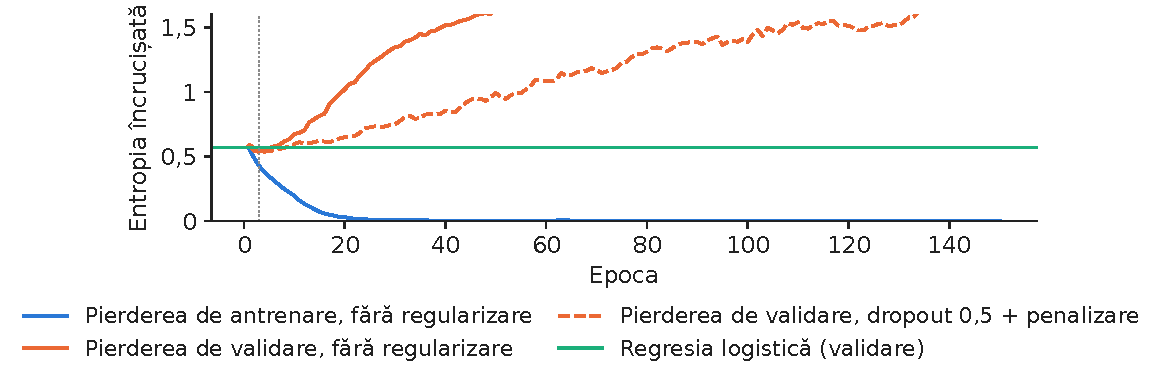
\includegraphics[width=\textwidth,height=0.331\textheight,keepaspectratio]{charts/ro/overfit_german.pdf}\end{center}\vspace{-3mm}
\chartsource{Sursa: UCI Machine Learning Repository, Statlog German credit. Date: 600 de solicitanți de antrenare și 200 de validare; MLP 256-256.}
\vspace{0.5mm}
\begin{itemize}\setlength{\itemsep}{0pt}
  \item Pierderea de validare 0{,}536 la epoca 3, 2{,}187 după 150
    \begin{itemize}\setlength{\itemsep}{0pt}
      \item Cu dropout și penalizare 1{,}767
      \item Logistic 0{,}570.
    \end{itemize}
\end{itemize}
\par\vfill\manager{o pierdere de antrenare aproape de zero pe date de credit este un semnal de alarmă.}\par\vspace{0.5mm}
\par\vfill\noindent{\scriptsize\color{FooterGray}(calcul propriu)}\hfill\qlink{NN\_L3\_overfit\_german}{Quantlets/L3/NN_L3_overfit_german}\par\vspace{0.5mm}
\end{frame}

\begin{frame}{Eroarea pe test se descompune în deplasare, varianță și zgomot}
\small
\intuition{un model rigid ratează tiparul (deplasare), unul flexibil urmărește zgomotul eșantionului său (varianță).}
\[ \E_{\mathcal D,\varepsilon}\big[(y-\hat f_{\mathcal D}(x))^2\big]=\underbrace{\big(f(x)-\E_{\mathcal D}\hat f_{\mathcal D}(x)\big)^2}_{\text{deplasare}^2}+\underbrace{\Var_{\mathcal D}\big(\hat f_{\mathcal D}(x)\big)}_{\text{varianță}}+\underbrace{\sigma^2}_{\text{zgomot}} \]
{\footnotesize\begin{itemize}\setlength{\itemsep}{0pt}
  \item \textbf{\txtwhere}
    \begin{itemize}\setlength{\itemsep}{0pt}
      \item $y=f(x)+\varepsilon$, $\Var(\varepsilon)=\sigma^2$, $\hat f_{\mathcal D}$ modelul estimat pe un eșantion aleator de antrenare $\mathcal D$, derivarea în anexă
    \end{itemize}
\end{itemize}\par}
\begin{itemize}\setlength{\itemsep}{2pt}
  \item Regularizarea acceptă puțină deplasare în schimbul unei reduceri mari a varianței
    \begin{itemize}\setlength{\itemsep}{0pt}
      \item Zgomotul $\sigma^2$ este o limită pe care niciun model nu o poate depăși.
    \end{itemize}
  \item Curba clasică în U: eroarea pe test întîi scade, apoi crește cu capacitatea
    \begin{itemize}\setlength{\itemsep}{0pt}
      \item Rețelele foarte mari pot avea o a doua coborîre (slide-ul următor).
    \end{itemize}
\end{itemize}
\par\vfill\manager{cu puține observații domină varianța: preferați modele simple sau regularizare puternică.}\par\vspace{0.5mm}
\par\vfill\noindent{\scriptsize\color{FooterGray}(Hastie, Tibshirani \& Friedman, 2009, ch.~7)}\par\vspace{0.5mm}
\end{frame}

\begin{frame}{După pragul de interpolare, mai mulți neuroni ascunși reduc din nou eroarea}
\small
\intuition{$p$ unități liniare rectificate (ReLU) aleatoare și fixe, ieșire de normă minimă, $n=$ 400 de grupuri.}
\begin{center}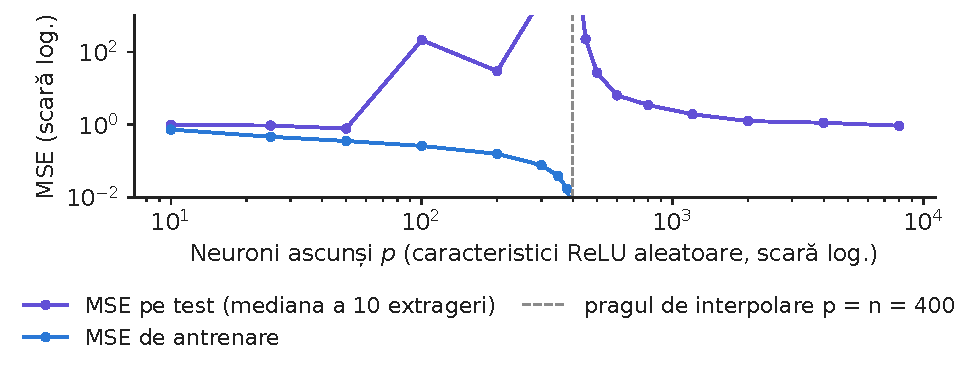
\includegraphics[width=\textwidth,height=0.342\textheight,keepaspectratio]{charts/ro/double_descent.pdf}\end{center}\vspace{-3mm}
\chartsource{Sursa: StatLib, locuințe din California, recensămîntul din 1990 (Pace și Barry, 1997). Date: 400 de grupuri de antrenare și 5\,000 de testare la fiecare extragere, 10 extrageri.}
\vspace{0.5mm}
\begin{itemize}\setlength{\itemsep}{0pt}
  \item Eroarea pătratică medie (MSE) pe test: 0{,}781 la $p=$ 50, $1{,}0\times10^{6}$ la $p=n$, 0{,}932 la $p=$ 8\,000 (mediana a 10 extrageri).
\end{itemize}
\par\vfill\manager{lîngă $p=n$, un model mai mare poate fi mult mai slab, mult după, mărimea ajută din nou.}\par\vspace{0.5mm}
\par\vfill\noindent{\scriptsize\color{FooterGray}(Belkin et al., 2019; Nakkiran et al., 2021)}\hfill\qlink{NN\_L3\_double\_descent}{Quantlets/L3/NN_L3_double_descent}\par\vspace{0.5mm}
\end{frame}


\section{Penalizarea ponderilor}

\begin{frame}{Penalizarea ponderilor = penalizare L2 = o distribuție a priori gaussiană pe ponderi}
\small
\intuition{ponderile mari fac funcția abruptă și sensibilă la zgomot; micșorarea lor o face mai netedă.}
\[ \tilde\loss(\vw)=\loss(\vw)+\frac\lambda2\|\vw\|_2^2\ \Rightarrow\ \vw_{t+1}=(1-\eta\lambda)\,\vw_t-\eta\nabla\loss(\vw_t);\qquad \vw\sim\mathcal N(\mathbf 0,\lambda^{-1}\mathbf I)\Rightarrow\hat\vw_{\mathrm{MAP}}=\argmin\tilde\loss \]
{\footnotesize\begin{itemize}\setlength{\itemsep}{0pt}
  \item \textbf{\txtwhere}
    \begin{itemize}\setlength{\itemsep}{0pt}
      \item $\lambda>0$ intensitatea penalizării, $(1-\eta\lambda)$ micșorarea la fiecare pas de coborîre stohastică pe gradient (SGD), estimarea maximum a posteriori (MAP)
    \end{itemize}
\end{itemize}\par}
\begin{itemize}\setlength{\itemsep}{2pt}
  \item În modelul liniar este regresia ridge: pe direcția proprie $k$, coeficienții sînt micșorați cu $\frac{d_k}{d_k+\lambda}$ (Hoerl \& Kennard, 1970).
  \item Cu Adam, termenul L2 este rescalat pe fiecare pondere
    \begin{itemize}\setlength{\itemsep}{0pt}
      \item Adam cu penalizare decuplată (AdamW) micșorează toate ponderile la fel (Loshchilov \& Hutter, 2019).
    \end{itemize}
\end{itemize}
\par\vfill\manager{penalizarea ponderilor este primul regularizator de ajustat
    \begin{itemize}\setlength{\itemsep}{0pt}
      \item Căutați $\lambda$ pe o grilă logaritmică, cu validare.
    \end{itemize}}\par\vspace{0.5mm}
\par\vfill\noindent{\scriptsize\color{FooterGray}(Bishop \& Bishop, 2024, ch.~9)}\hfill\tryit{notebook \S3}\par\vspace{0.5mm}
\end{frame}

\begin{frame}{O penalizare L1 aduce ponderile exact la zero}
\small
\intuition{bila L1 are colțuri pe axe, deci optimul penalizat cade adesea într-unul: rezultă un model rar (sparse).}
\[ \tilde\loss(\vw)=\loss(\vw)+\lambda\|\vw\|_1,\qquad \text{pasul proximal: }\ w_j\leftarrow\operatorname{sign}(u_j)\max\big(|u_j|-\eta\lambda,0\big),\ u_j=w_j-\eta\,\partial_j\loss \]
{\footnotesize\begin{itemize}\setlength{\itemsep}{0pt}
  \item \textbf{\txtwhere}
    \begin{itemize}\setlength{\itemsep}{0pt}
      \item $\|\vw\|_1=\sum_j|w_j|$, pasul de prag moale aduce ponderile mici exact la zero (lasso, Tibshirani, 1996)
    \end{itemize}
\end{itemize}\par}
\begin{itemize}\setlength{\itemsep}{2pt}
  \item L1 pe primul strat al unui MLP acționează ca selecție de variabile: o intrare ale cărei ponderi spre stratul ascuns sînt toate zero este oprită.
  \item Elastic net le combină: $\lambda_1\|\vw\|_1+\tfrac{\lambda_2}2\|\vw\|_2^2$.
\end{itemize}
\par\vfill\manager{folosiți L1 cînd documentația modelului cere o listă scurtă de intrări.}\par\vspace{0.5mm}
\par\vfill\noindent{\scriptsize\color{FooterGray}(Tibshirani, 1996)}\hfill\tryit{notebook \S3}\par\vspace{0.5mm}
\end{frame}

\begin{frame}{L1 adună ponderile primului strat în zero, L2 doar le micșorează}
\small
\intuition{MLP cu 64 de neuroni ascunși pe German credit, Adam pe tot setul, penalizare doar pe primul strat.}
\begin{center}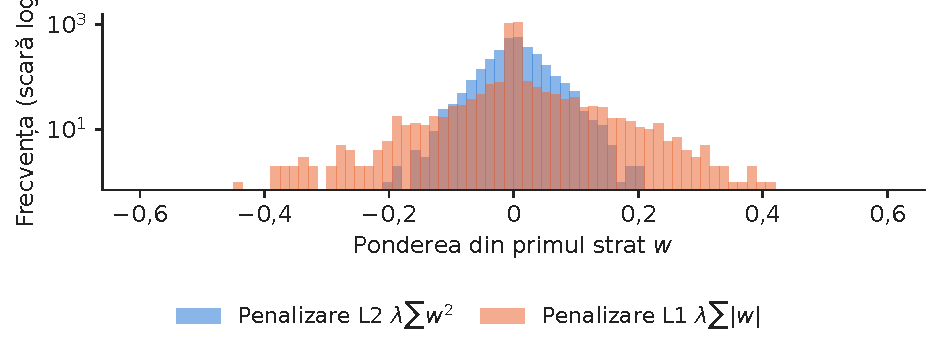
\includegraphics[width=\textwidth,height=0.356\textheight,keepaspectratio]{charts/ro/l1_l2_weights.pdf}\end{center}\vspace{-3mm}
\chartsource{Sursa: UCI Machine Learning Repository, Statlog German credit. Date: 600 de solicitanți de antrenare; MLP cu 64 de neuroni ascunși\, 3\,072 de ponderi în primul strat.}
\vspace{0.5mm}
\begin{itemize}\setlength{\itemsep}{0pt}
  \item Ponderi cu $|w|<$ 0{,}01: 67{,}2\,\% cu L1 față de 26{,}3\,\% cu L2 (3\,072 de ponderi)
    \begin{itemize}\setlength{\itemsep}{0pt}
      \item AUC pe test 0{,}768 cu L1, față de 0{,}761 cu L2.
    \end{itemize}
\end{itemize}
\par\vfill\manager{o penalizare L1 mai puternică ar anula coloane întregi de intrări, care pot ieși apoi din fluxul de date.}\par\vspace{0.5mm}
\par\vfill\noindent{\scriptsize\color{FooterGray}(calcul propriu)}\hfill\qlink{NN\_L3\_l1\_l2\_weights}{Quantlets/L3/NN_L3_l1_l2_weights}\par\vspace{0.5mm}
\end{frame}


\section{Dropout, oprirea timpurie și normalizarea pe loturi}

\begin{frame}{Dropout antrenează un ansamblu de rețele subțiate care își împart ponderile}
\small
\intuition{oprirea aleatoare a unor neuroni împiedică orice neuron să depindă de cîțiva alții: fiecare variabilă trebuie să fie utilă singură.}
\[ \text{antrenare: }\ \tilde h_j=\frac{m_j}{1-p}\,h_j,\ \ m_j\iid\text{Bernoulli}(1-p);\qquad \text{test: }\ \tilde h_j=h_j \]
{\footnotesize\begin{itemize}\setlength{\itemsep}{0pt}
  \item \textbf{\txtwhere}
    \begin{itemize}\setlength{\itemsep}{0pt}
      \item $p$ rata de dropout, $m_j$ masca aleatoare, împărțirea la $1-p$ (dropout inversat) păstrează $\E[\tilde h_j]=h_j$, deci nimic nu se schimbă la testare
    \end{itemize}
\end{itemize}\par}
\begin{itemize}\setlength{\itemsep}{2pt}
  \item Cu $H$ neuroni care pot fi opriți, eșantionăm din $2^H$ subrețele
    \begin{itemize}\setlength{\itemsep}{0pt}
      \item La testare, rețeaua completă aproximează media lor (Srivastava et al., 2014).
    \end{itemize}
  \item Rate uzuale: 0,1--0,3 în MLP tabelare, 0,5 în straturile mari
    \begin{itemize}\setlength{\itemsep}{0pt}
      \item În PyTorch, \texttt{model.eval()} îl dezactivează.
    \end{itemize}
\end{itemize}
\par\vfill\manager{dacă uitați \texttt{model.eval()} înainte de scorare, fiecare predicție devine aleatoare.}\par\vspace{0.5mm}
\par\vfill\noindent{\scriptsize\color{FooterGray}(Srivastava et al., 2014)}\hfill\tryit{notebook \S4}\par\vspace{0.5mm}
\end{frame}

\begin{frame}{Pe 600 de solicitanți, regularizarea nu egalează regresia logistică}
\small
\intuition{MLP 256-256, 150 de epoci fără oprire timpurie; AUC pe pliul de test, 5 pliuri, pentru fiecare $\lambda$ și $p$.}
\begin{center}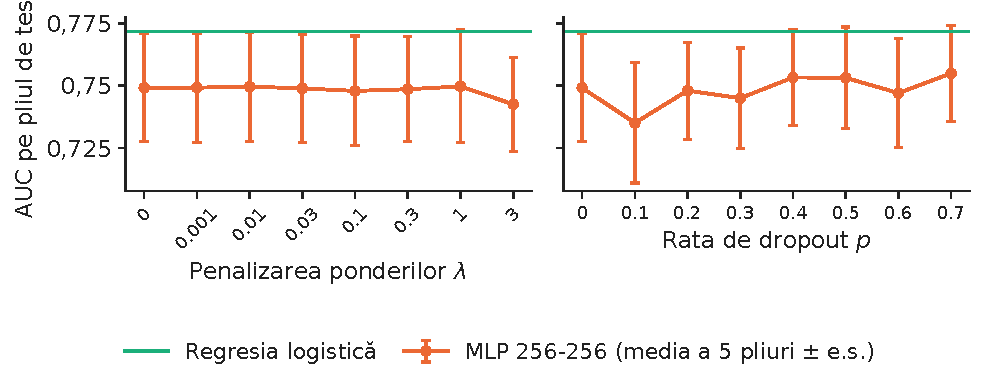
\includegraphics[width=\textwidth,height=0.321\textheight,keepaspectratio]{charts/ro/wd_dropout.pdf}\end{center}\vspace{-3mm}
\chartsource{Sursa: UCI Machine Learning Repository, Statlog German credit. Date: 1\,000 de solicitanți, validare încrucișată cu 5 pliuri, fără oprire timpurie (150 de epoci).}
\vspace{0.5mm}
\begin{itemize}\setlength{\itemsep}{0pt}
  \item AUC 0{,}749 fără regularizare, 0{,}750 la $\lambda=$ 1, 0{,}755 la $p=$ 0{,}7
    \begin{itemize}\setlength{\itemsep}{0pt}
      \item Logistic 0{,}772
      \item Norma ponderilor 18{,}0 față de 10{,}6 la $\lambda=3$.
    \end{itemize}
\end{itemize}
\par\vfill\manager{pe date foarte puține, un model mai mic depășește unul mare regularizat.}\par\vspace{0.5mm}
\par\vfill\noindent{\scriptsize\color{FooterGray}(calcul propriu)}\hfill\qlink{NN\_L3\_wd\_dropout}{Quantlets/L3/NN_L3_wd_dropout}\par\vspace{0.5mm}
\end{frame}

\begin{frame}{Oprirea timpurie: păstrăm ponderile epocii celei mai bune pe validare}
\small
\intuition{o antrenare mai lungă potrivește mai mult zgomot; ne oprim cînd pierderea de validare nu s-a mai îmbunătățit de ceva timp.}
\[ t^*=\argmin_{t\le T}\ \loss_{\text{val}}(\vw_t),\quad \text{oprire cînd}\ t-t^*\ge P;\qquad \text{pierdere pătratică:}\ \ \eta\,t\ \approx\ \frac1\lambda \]
{\footnotesize\begin{itemize}\setlength{\itemsep}{0pt}
  \item \textbf{\txtwhere}
    \begin{itemize}\setlength{\itemsep}{0pt}
      \item $P$ răbdarea, în epoci, ultima relație spune că $t$ pași de mărime $\eta$ acționează ca o penalizare L2 de intensitate $\lambda\approx1/(\eta t)$ (anexa)
    \end{itemize}
\end{itemize}\par}
\begin{itemize}\setlength{\itemsep}{2pt}
  \item Setul de validare este folosit pentru decizia de oprire: nu mai este o estimare nedeplasată, deci este nevoie de un set de test separat.
  \item Este gratuită, ieftină și compatibilă cu orice alt regularizator (Prechelt, 1998).
\end{itemize}
\par\vfill\manager{salvați cea mai bună stare a modelului, nu ultima.}\par\vspace{0.5mm}
\par\vfill\noindent{\scriptsize\color{FooterGray}(Prechelt, 1998; Bishop \& Bishop, 2024, ch.~9)}\hfill\tryit{notebook \S5}\par\vspace{0.5mm}
\end{frame}

\begin{frame}{La fraude, pierderea de validare atinge minimul devreme, cea de antrenare tot scade}
\small
\intuition{MLP 256-256, împărțire cronologică; punctat: epoca cea mai bună pe validare; gri: fereastra de răbdare.}
\begin{center}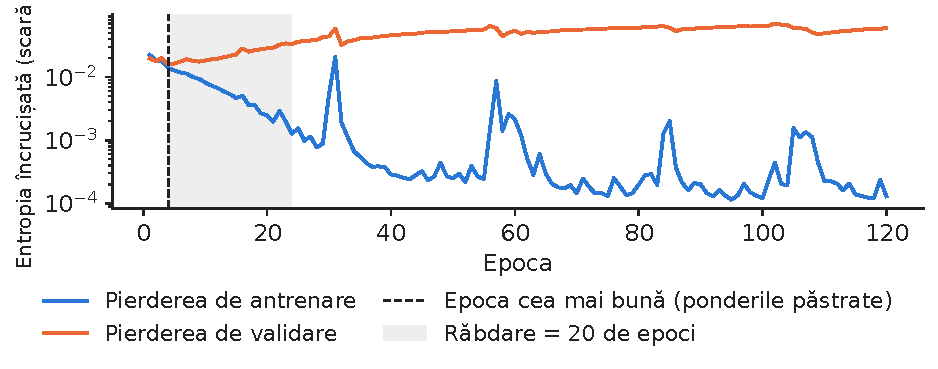
\includegraphics[width=\textwidth,height=0.310\textheight,keepaspectratio]{charts/ro/early_stopping.pdf}\end{center}\vspace{-3mm}
\chartsource{Sursa: ULB Machine Learning Group și Worldline, tranzacții cu carduri (OpenML 1597). Date: împărțire cronologică: 17\,354 de tranzacții de antrenare\, 5\,785 de validare.}
\vspace{0.5mm}
\begin{itemize}\setlength{\itemsep}{0pt}
  \item Epoca cea mai bună 4, oprire la 24 (răbdare 20)
    \begin{itemize}\setlength{\itemsep}{0pt}
      \item Pierderea de validare 0{,}0159 atunci, 0{,}0593 după 120 de epoci.
    \end{itemize}
\end{itemize}
\par\vfill\manager{la evenimente rare, rețeaua începe să memoreze puținele fraude de antrenare după cîteva epoci.}\par\vspace{0.5mm}
\par\vfill\noindent{\scriptsize\color{FooterGray}(calcul propriu)}\hfill\qlink{NN\_L3\_early\_stopping}{Quantlets/L3/NN_L3_early_stopping}\par\vspace{0.5mm}
\end{frame}

\begin{frame}{Normalizarea pe loturi standardizează fiecare neuron pe mini-lot}
\small
\intuition{păstrarea preactivărilor centrate și scalate permite rețelelor adînci să se antreneze cu pași mai mari.}
\[ \hat z_{ij}=\frac{z_{ij}-\mu_{\mathcal B,j}}{\sqrt{\sigma^2_{\mathcal B,j}+\epsilon}},\qquad y_{ij}=\gamma_j\hat z_{ij}+\beta_j,\qquad \mu_{\mathcal B,j}=\frac1B\sum_{i\in\mathcal B}z_{ij} \]
{\footnotesize\begin{itemize}\setlength{\itemsep}{0pt}
  \item \textbf{\txtwhere}
    \begin{itemize}\setlength{\itemsep}{0pt}
      \item $\sigma^2_{\mathcal B,j}$ varianța pe lot a neuronului $j$, $\gamma_j,\beta_j$ scara și deplasarea învățate, la testare, mediile mobile înlocuiesc statisticile lotului
    \end{itemize}
\end{itemize}\par}
\begin{itemize}\setlength{\itemsep}{2pt}
  \item Normalizarea pe loturi (BN) netezește suprafața pierderii, ceea ce permite rate de învățare mai mari (Ioffe \& Szegedy, 2015).
  \item Statisticile lotului adaugă zgomot la ieșirea fiecărui exemplu: un regularizator slab
    \begin{itemize}\setlength{\itemsep}{0pt}
      \item Normalizarea pe strat (cursul 7) evită dependența de lot.
    \end{itemize}
\end{itemize}
\par\vfill\manager{cu normalizare pe loturi, \texttt{model.eval()} este obligatoriu, iar loturile foarte mici trebuie evitate.}\par\vspace{0.5mm}
\par\vfill\noindent{\scriptsize\color{FooterGray}(Ioffe \& Szegedy, 2015)}\hfill\tryit{notebook \S6}\par\vspace{0.5mm}
\end{frame}

\begin{frame}{Normalizarea pe loturi permite antrenarea la o rată la care altfel rețeaua diverge}
\small
\intuition{6 straturi ascunse de 64 de neuroni pe California housing, SGD cu moment; mediane a 3 inițializări.}
\begin{center}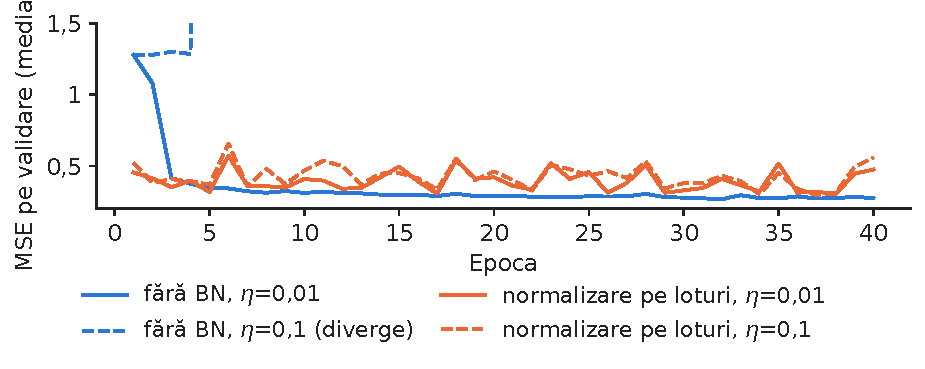
\includegraphics[width=\textwidth,height=0.306\textheight,keepaspectratio]{charts/ro/batchnorm.pdf}\end{center}\vspace{-3mm}
\chartsource{Sursa: StatLib, locuințe din California, recensămîntul din 1990 (Pace și Barry, 1997). Date: 6 straturi ascunse de 64 de neuroni, SGD cu moment 0,9, 3 inițializări.}
\vspace{0.5mm}
\begin{itemize}\setlength{\itemsep}{0pt}
  \item La $\eta=0{,}1$: 3 din 3 inițializări diverg fără BN, cea mai bună MSE pe validare 0{,}283 cu BN
    \begin{itemize}\setlength{\itemsep}{0pt}
      \item La $\eta=0{,}01$: 0{,}265 fără, 0{,}277 cu BN.
    \end{itemize}
\end{itemize}
\par\vfill\manager{normalizarea pe loturi ajută mai ales optimizarea
    \begin{itemize}\setlength{\itemsep}{0pt}
      \item Păstrați oprirea timpurie, eroarea ei fluctuează.
    \end{itemize}}\par\vspace{0.5mm}
\par\vfill\noindent{\scriptsize\color{FooterGray}(calcul propriu)}\hfill\qlink{NN\_L3\_batchnorm}{Quantlets/L3/NN_L3_batchnorm}\par\vspace{0.5mm}
\end{frame}

\begin{frame}{Alți regularizatori: mai multe date, zgomot, ansambluri}
\small
\begin{columns}[T,onlytextwidth]
\begin{column}{0.50\textwidth}
\begin{itemize}\setlength{\itemsep}{2pt}
  \item \textbf{Augmentarea datelor}: transformări care păstrează eticheta (decupări și oglindiri pentru imagini, cursul 4)
    \begin{itemize}\setlength{\itemsep}{0pt}
      \item Pentru date tabelare, rareori sigură.
    \end{itemize}
  \item \textbf{Injectarea de zgomot}: zgomotul gaussian pe intrări este echivalent, în prima aproximare, cu o penalizare L2 a gradientului în raport cu intrările.
  \item \textbf{Netezirea etichetelor}: antrenăm pe $(1-\epsilon)y+\epsilon/2$ în loc de ținte 0/1
    \begin{itemize}\setlength{\itemsep}{0pt}
      \item Limitează probabilitățile prea sigure.
    \end{itemize}
\end{itemize}
\end{column}
\begin{column}{0.47\textwidth}
\begin{itemize}\setlength{\itemsep}{2pt}
  \item \textbf{Ansamblurile}: media mai multor inițializări sau modele
    \begin{itemize}\setlength{\itemsep}{0pt}
      \item Varianța scade aproximativ ca $1/M$ pentru $M$ membri slab corelați.
    \end{itemize}
  \item \textbf{Un model mai mic sau mai puține intrări}: cel mai vechi regularizator.
  \item \textbf{Mai multe date}: singurul fără efecte secundare
    \begin{itemize}\setlength{\itemsep}{0pt}
      \item Încă un an de tranzacții valorează mai mult decît orice penalizare.
    \end{itemize}
\end{itemize}
\end{column}
\end{columns}
\par\vfill\manager{studiul de caz despre fraudă face media a 5 inițializări: un ansamblu ieftin care raportează și incertitudinea.}\par\vspace{0.5mm}
\par\vfill\noindent{\scriptsize\color{FooterGray}(Bishop \& Bishop, 2024, ch.~9)}\par\vspace{0.5mm}
\end{frame}


\section{Schema de validare}

\begin{frame}{Setul păstrat deoparte, validarea încrucișată și validarea încrucișată imbricată}
\small
\intuition{orice alegere făcută privind datele trebuie plătită cu date pe care alegerea nu le-a văzut.}
\[ \widehat{\mathrm{CV}}_K=\frac1K\sum_{k=1}^{K}\frac1{|\mathcal D_k|}\sum_{i\in\mathcal D_k}\ell\big(y_i,\hat f^{(-k)}(\vx_i)\big) \]
{\footnotesize\begin{itemize}\setlength{\itemsep}{0pt}
  \item \textbf{\txtwhere}
    \begin{itemize}\setlength{\itemsep}{0pt}
      \item $\mathcal D_k$ pliul $k$, $\hat f^{(-k)}$ modelul estimat pe celelalte $K-1$ pliuri, de obicei $K=5$ sau 10, stratificat după etichetă
    \end{itemize}
\end{itemize}\par}
\begin{itemize}\setlength{\itemsep}{2pt}
  \item Setul păstrat deoparte: o singură împărțire antrenare/validare/test
    \begin{itemize}\setlength{\itemsep}{0pt}
      \item Ieftin, dar zgomotos pe date puține (slide-ul următor).
    \end{itemize}
  \item Validarea încrucișată imbricată: o buclă interioară ajustează hiperparametrii, una exterioară măsoară întreaga procedură de ajustare.
  \item Raportați variația între pliuri, nu doar media
    \begin{itemize}\setlength{\itemsep}{0pt}
      \item Comparați modelele cu testul $t$ corectat din cursul 1.
    \end{itemize}
\end{itemize}
\par\vfill\manager{performanța raportată trebuie să provină din date folosite nici la estimare, nici la alegere.}\par\vspace{0.5mm}
\par\vfill\noindent{\scriptsize\color{FooterGray}(Hastie, Tibshirani \& Friedman, 2009, ch.~7)}\hfill\tryit{notebook \S7}\par\vspace{0.5mm}
\end{frame}

\begin{frame}{O singură împărțire aleatoare poate muta AUC cu cîteva puncte}
\small
\intuition{regresia logistică pe German credit, 200 de împărțiri aleatoare stratificate 70/30 ale acelorași solicitanți.}
\begin{center}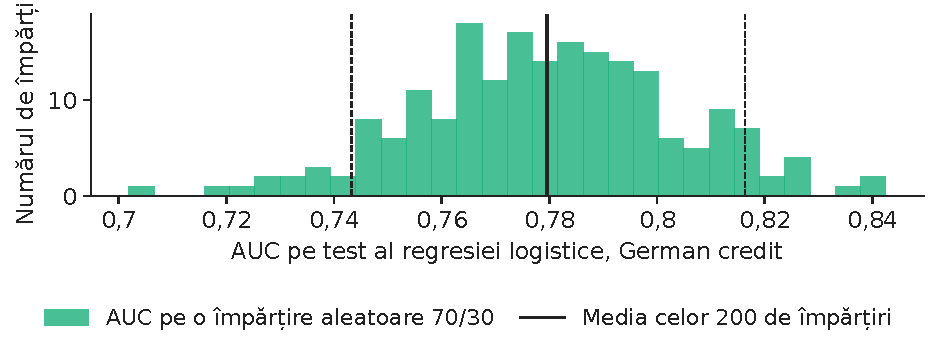
\includegraphics[width=\textwidth,height=0.389\textheight,keepaspectratio]{charts/ro/holdout_noise.pdf}\end{center}\vspace{-3mm}
\chartsource{Sursa: UCI Machine Learning Repository, Statlog German credit. Date: 1\,000 de solicitanți, 200 de împărțiri aleatoare stratificate.}
\vspace{0.5mm}
\begin{itemize}\setlength{\itemsep}{0pt}
  \item AUC pe test între 0{,}702 și 0{,}842
    \begin{itemize}\setlength{\itemsep}{0pt}
      \item 90\,\% dintre împărțiri în [0{,}743; 0{,}816], abaterea standard 0{,}024.
    \end{itemize}
\end{itemize}
\par\vfill\manager{pe un set mic, o singură împărțire nu poate separa două modele: folosiți validarea încrucișată repetată.}\par\vspace{0.5mm}
\par\vfill\noindent{\scriptsize\color{FooterGray}(calcul propriu)}\hfill\qlink{NN\_L3\_holdout\_noise}{Quantlets/L3/NN_L3_holdout_noise}\par\vspace{0.5mm}
\end{frame}

\begin{frame}{Scurgerea de informație: cînd setul de validare știe ceva ce nu ar trebui}
\small
\intuition{orice informație din rîndurile de evaluare care ajunge în antrenare umflă scorul și dispare în producție.}
{\scriptsize\renewcommand{\arraystretch}{1.05}\setlength{\tabcolsep}{4pt}
\begin{tabular}{@{}p{0.27\textwidth}p{0.36\textwidth}p{0.30\textwidth}@{}}\toprule
Scurgerea & Exemplu & Remediu \\ \midrule
Preprocesare pe toate rîndurile & standardizare sau completare estimate înainte de împărțire & estimare doar pe antrenare \\
Reeșantionare înainte de împărțire & copii ale unei fraude în antrenare și în test & supraeșantionare doar în pliul de antrenare \\
Ignorarea timpului & împărțire aleatoare a unei serii de timp sau a plăților & antrenare pe trecut, testare pe viitor \\
Ținta în intrări & „zile de întîrziere” folosite pentru a prezice neplata & doar informații cunoscute la momentul deciziei \\
\bottomrule\end{tabular}}
\par\vspace{0.5mm}{\scriptsize \begin{itemize}\setlength{\itemsep}{0pt}
  \item Serii de timp: validare cu fereastră extinsă sau pe blocuri; nu amestecați niciodată ordinea (Bergmeir \& Benítez, 2012).
\end{itemize}}
\par\vfill\manager{notați, pentru fiecare intrare, momentul în care devine cunoscută.}\par\vspace{0.5mm}
\par\vfill\noindent{\scriptsize\color{FooterGray}(Kaufman et al., 2012)}\hfill\tryit{notebook \S8}\par\vspace{0.5mm}
\end{frame}

\begin{frame}{Supraeșantionarea înainte de împărțire face un detector să pară mult mai bun, pe hîrtie}
\small
\intuition{același MLP 128-128 și aceleași tranzacții, evaluate în trei moduri; cîte 5 inițializări.}
\begin{center}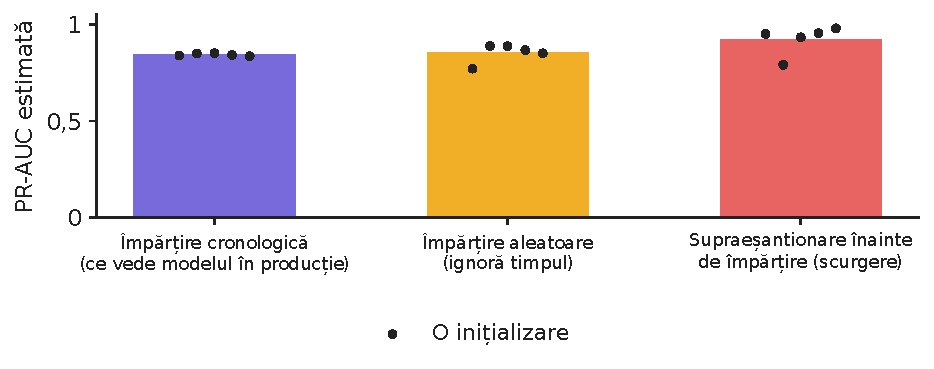
\includegraphics[width=\textwidth,height=0.333\textheight,keepaspectratio]{charts/ro/split_leakage.pdf}\end{center}\vspace{-3mm}
\chartsource{Sursa: ULB Machine Learning Group și Worldline, tranzacții cu carduri (OpenML 1597). Date: aceleași 28\,924 de tranzacții, MLP 128-128 cu oprire timpurie, 5 inițializări.}
\vspace{0.5mm}
\begin{itemize}\setlength{\itemsep}{0pt}
  \item PR-AUC 0{,}843 cu împărțire cronologică, 0{,}853 cu împărțire aleatoare, 0{,}921 cu fraudele copiate de 20 de ori înainte de împărțire.
\end{itemize}
\par\vfill\manager{doar estimarea cronologică descrie ce va vedea banca după punerea în producție.}\par\vspace{0.5mm}
\par\vfill\noindent{\scriptsize\color{FooterGray}(calcul propriu)}\hfill\qlink{NN\_L3\_split\_leakage}{Quantlets/L3/NN_L3_split_leakage}\par\vspace{0.5mm}
\end{frame}


\section{Studiu de caz: detectarea fraudei cu carduri}

\begin{frame}{Frauda este rară și grupată în timp}
\small
\intuition{datele Université libre de Bruxelles (ULB) și Worldline, platforma Open Machine Learning (OpenML): două zile de plăți cu cardul.}
\begin{center}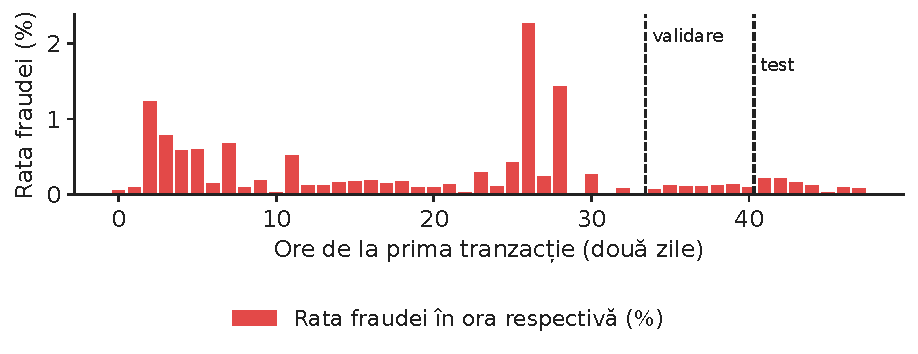
\includegraphics[width=\textwidth,height=0.321\textheight,keepaspectratio]{charts/ro/fraud_by_hour.pdf}\end{center}\vspace{-3mm}
\chartsource{Sursa: ULB Machine Learning Group și Worldline, tranzacții cu carduri (OpenML 1597). Date: septembrie 2013, 2 zile, 284\,807 tranzacții (eșantion ponderat).}
\vspace{0.5mm}
\begin{itemize}\setlength{\itemsep}{0pt}
  \item 284\,807 de plăți, rata fraudei 0{,}173\,\%
    \begin{itemize}\setlength{\itemsep}{0pt}
      \item Păstrăm toate cele 492 de fraude și 10\,\% din plățile legitime (ponderea 10)
      \item Intrări: 28 de scoruri de analiză a componentelor principale (PCA) și logaritmul sumei.
    \end{itemize}
\end{itemize}
\par\vfill\manager{rata orară variază puternic: o împărțire aleatoare ar amesteca orele liniștite și cele de atac.}\par\vspace{0.5mm}
\par\vfill\noindent{\scriptsize\color{FooterGray}(Dal Pozzolo et al., 2015)}\hfill\qlink{NN\_L3\_fraud\_by\_hour}{Quantlets/L3/NN_L3_fraud_by_hour}\par\vspace{0.5mm}
\end{frame}

\begin{frame}{La evenimente rare, acuratețea este inutilă: măsurăm precizia, sensibilitatea și PR-AUC}
\small
\intuition{dacă nu semnalăm nimic avem o acuratețe de 99,8\,\%; banca vrea să știe cîte alerte sînt fraude și cîte fraude declanșează o alertă.}
\[ \text{precizia}=\frac{TP}{TP+FP},\quad \text{sensibilitatea}=\frac{TP}{TP+FN},\quad \text{PR-AUC}=\sum_k(R_k-R_{k-1})\,P_k \]
{\footnotesize\begin{itemize}\setlength{\itemsep}{0pt}
  \item \textbf{\txtwhere}
    \begin{itemize}\setlength{\itemsep}{0pt}
      \item $TP$, $FP$, $FN$ adevărat pozitive, fals pozitive, fals negative la un prag, $P_k,R_k$ precizia și sensibilitatea la al $k$-lea prag
    \end{itemize}
\end{itemize}\par}
\begin{itemize}\setlength{\itemsep}{2pt}
  \item PR-AUC depinde de rata fraudei (un scor aleator are PR-AUC = rata fraudei)
    \begin{itemize}\setlength{\itemsep}{0pt}
      \item AUC nu depinde, ceea ce ascunde alarmele false (Saito \& Rehmsmeier, 2015).
    \end{itemize}
  \item Date subeșantionate: fiecare plată legitimă contează cu ponderea 10{,}00 în $FP$, deci precizia este cea a populației complete.
\end{itemize}
\par\vfill\manager{raportați precizia la sensibilitatea pe care o poate gestiona echipa de investigații.}\par\vspace{0.5mm}
\par\vfill\noindent{\scriptsize\color{FooterGray}(Saito \& Rehmsmeier, 2015)}\hfill\tryit{notebook \S9}\par\vspace{0.5mm}
\end{frame}

\begin{frame}{Pe orele de test, oprirea timpurie este regularizatorul care ajută clar}
\small
\intuition{MLP 256-256, împărțire cronologică, 5 inițializări pe configurație; precizia ponderată la populație.}
\begin{center}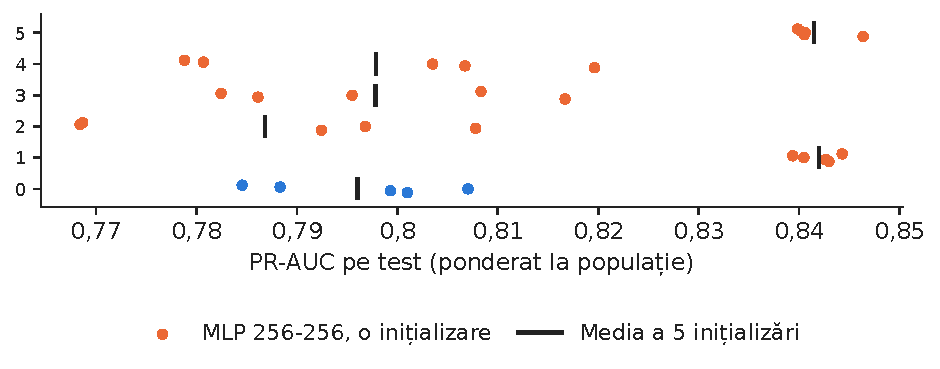
\includegraphics[width=\textwidth,height=0.379\textheight,keepaspectratio]{charts/ro/reg_ablation.pdf}\end{center}\vspace{-3mm}
\chartsource{Sursa: ULB Machine Learning Group și Worldline, tranzacții cu carduri (OpenML 1597). Date: setul de test cronologic: ultimele 5\,785 de tranzacții (75 de fraude); 5 inițializări.}
\vspace{0.5mm}
\begin{itemize}\setlength{\itemsep}{0pt}
  \item PR-AUC pe test: nimic 0{,}796, oprire timpurie 0{,}842, penalizare 0{,}787, dropout 0{,}798, normalizare 0{,}798, toate 0{,}841.
\end{itemize}
\par\vfill\manager{cu 60 de epoci fixe, ceilalți regularizatori rămîn în zgomotul inițializărilor.}\par\vspace{0.5mm}
\par\vfill\noindent{\scriptsize\color{FooterGray}(calcul propriu)}\hfill\qlink{NN\_L3\_reg\_ablation}{Quantlets/L3/NN_L3_reg_ablation}\par\vspace{0.5mm}
\end{frame}

\begin{frame}{Față de regresia logistică și gradient boosting, MLP regularizat se descurcă bine}
\small
\intuition{orele de test (ultimele 20\,\%); MLP mediază 5 inițializări cu oprire timpurie, penalizare și dropout.}
\begin{center}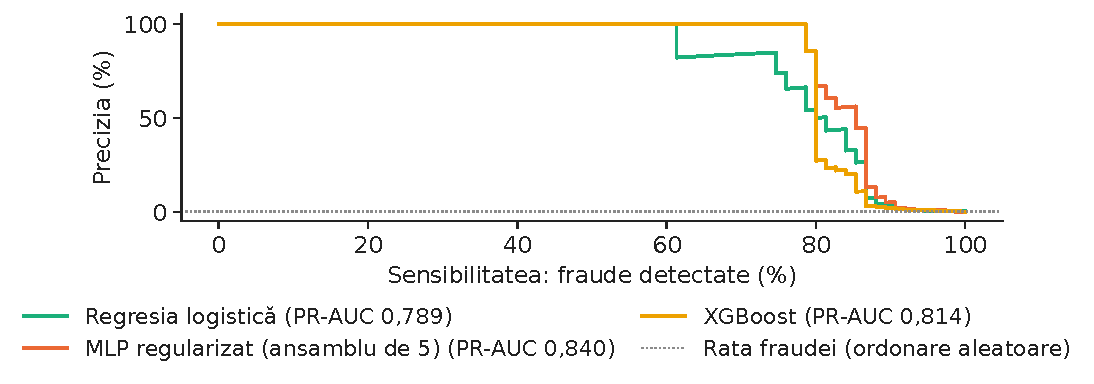
\includegraphics[width=\textwidth,height=0.397\textheight,keepaspectratio]{charts/ro/fraud_pr.pdf}\end{center}\vspace{-3mm}
\chartsource{Sursa: ULB Machine Learning Group și Worldline, tranzacții cu carduri (OpenML 1597). Date: setul de test cronologic: 5\,785 de tranzacții\, 75 de fraude\, ponderat la populație.}
\vspace{0.5mm}
\begin{itemize}\setlength{\itemsep}{0pt}
  \item PR-AUC: logistic 0{,}789, MLP 0{,}840, extreme gradient boosting (XGBoost) 0{,}814
    \begin{itemize}\setlength{\itemsep}{0pt}
      \item Sensibilitatea la precizie de 80\,\%: 74{,}7, 80{,}0, 80{,}0\,\%.
    \end{itemize}
\end{itemize}
\par\vfill\manager{cu 75 de fraude în test, cîteva puncte de diferență sînt în interiorul zgomotului.}\par\vspace{0.5mm}
\par\vfill\noindent{\scriptsize\color{FooterGray}(calcul propriu)}\hfill\qlink{NN\_L3\_fraud\_pr}{Quantlets/L3/NN_L3_fraud_pr}\par\vspace{0.5mm}
\end{frame}

\begin{frame}{Ponderile claselor și corecția pentru datele subeșantionate}
\small
\intuition{ponderarea clasei rare schimbă nivelul scorurilor, nu doar ordinea lor; după subeșantionare, probabilitățile trebuie corectate.}
\[ \loss_w=-\frac1n\sum_i\big[w_+\,y_i\log p_i+w_-\,(1-y_i)\log(1-p_i)\big],\qquad p=\frac{\beta\,p_s}{\beta\,p_s-p_s+1} \]
{\footnotesize\begin{itemize}\setlength{\itemsep}{0pt}
  \item \textbf{\txtwhere}
    \begin{itemize}\setlength{\itemsep}{0pt}
      \item $w_\pm$ ponderile claselor, $p_s$ probabilitatea învățată pe date în care plățile legitime au fost păstrate cu rata $\beta$ (aici 0,1), $p$ probabilitatea corectată
    \end{itemize}
\end{itemize}\par}
\begin{itemize}\setlength{\itemsep}{2pt}
  \item Ponderile claselor sau reeșantionarea schimbă pragul efectiv
    \begin{itemize}\setlength{\itemsep}{0pt}
      \item Ordonarea, deci și PR-AUC, se schimbă puțin.
    \end{itemize}
  \item Orice am face, pragul trebuie să provină din costuri (slide-ul următor), iar probabilitățile trebuie corectate înainte de a fi folosite ca atare.
\end{itemize}
\par\vfill\manager{nu raportați niciodată probabilități dintr-un model reeșantionat fără corecția pentru distribuția a priori.}\par\vspace{0.5mm}
\par\vfill\noindent{\scriptsize\color{FooterGray}(Dal Pozzolo et al., 2015)}\hfill\tryit{notebook \S10}\par\vspace{0.5mm}
\end{frame}

\begin{frame}{Numărul potrivit de alerte salvează cea mai mare parte din pierderi}
\small
\intuition{o fraudă ratată costă suma ei; fiecare alertă costă o verificare de 5 euro (EUR), o constantă aleasă a priori.}
\begin{center}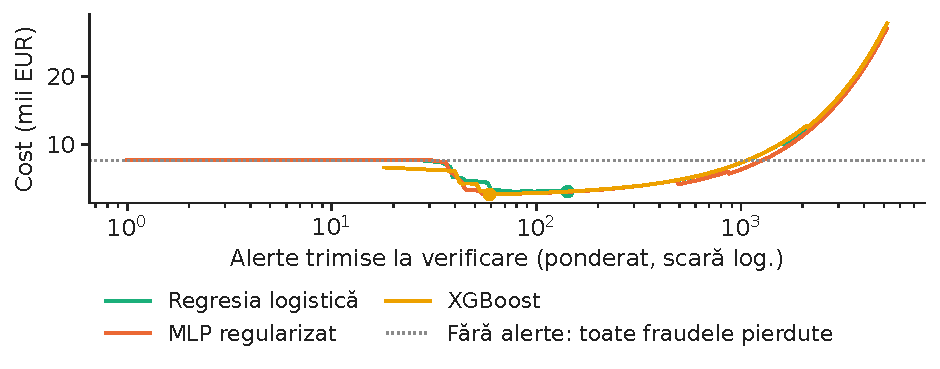
\includegraphics[width=\textwidth,height=0.398\textheight,keepaspectratio]{charts/ro/fraud_cost.pdf}\end{center}\vspace{-3mm}
\chartsource{Sursa: ULB Machine Learning Group și Worldline, tranzacții cu carduri (OpenML 1597). Date: perioada de test (ultimele 20\,\% din cele două zile); costul verificării 5 EUR pe alertă.}
\vspace{0.5mm}
\begin{itemize}\setlength{\itemsep}{0pt}
  \item Pierderi fără alerte 7\,729 EUR
    \begin{itemize}\setlength{\itemsep}{0pt}
      \item La numărul optim de alerte: logistic 3\,093, MLP 2\,694, XGBoost 2\,695 EUR.
    \end{itemize}
\end{itemize}
\par\vfill\manager{bugetul de alerte este decizia de afaceri, modelul doar ordonează.}\par\vspace{0.5mm}
\par\vfill\noindent{\scriptsize\color{FooterGray}(calcul propriu)}\hfill\qlink{NN\_L3\_fraud\_cost}{Quantlets/L3/NN_L3_fraud_cost}\par\vspace{0.5mm}
\end{frame}

\begin{frame}{Trusa de regularizare pe scurt}
\small
{\scriptsize\renewcommand{\arraystretch}{1.05}\setlength{\tabcolsep}{4pt}
\begin{tabular}{@{}p{0.17\textwidth}p{0.30\textwidth}p{0.22\textwidth}p{0.25\textwidth}@{}}\toprule
Metoda & Ce face & Parametrul principal & Pe datele noastre \\ \midrule
Penalizarea ponderilor & micșorează toate ponderile & $\lambda$ & ponderi mai mici, aceeași AUC (German) \\
L1 & aduce ponderi la zero & $\lambda$ & majoritatea ponderilor primului strat aproape de zero \\
Dropout & antrenează un ansamblu de subrețele & $p$ & în zgomotul inițializărilor \\
Oprirea timpurie & se oprește înainte de memorare & răbdarea $P$ & cîștig clar la fraudă \\
Normalizarea pe loturi & stabilizează antrenarea & mărimea lotului & învață la $\eta$ la care SGD simplu diverge \\
Model mai mic & mai puțini parametri & lățime, adîncime & regresia logistică depășește MLP pe German credit \\
\bottomrule\end{tabular}}
\par\vfill\manager{porniți cu oprirea timpurie și un model modest, apoi ajustați penalizarea
    \begin{itemize}\setlength{\itemsep}{0pt}
      \item Adăugați dropout și normalizare pe loturi la rețelele adînci.
    \end{itemize}}\par\vspace{0.5mm}
\end{frame}


\section{Sinteză}

\begin{frame}{Idei principale}
\small
\begin{itemize}\setlength{\itemsep}{4pt}
  \item Supraînvățarea apare ca o pierdere de antrenare care scade și o pierdere de validare care crește
    \begin{itemize}\setlength{\itemsep}{0pt}
      \item Pe date puține începe după cîteva epoci.
    \end{itemize}
  \item Penalizarea ponderilor (distribuție a priori gaussiană), L1 (raritate), dropout (ansamblu), oprirea timpurie (L2 implicit) și normalizarea pe loturi (ajutor la optimizare) controlează capacitatea în moduri diferite.
  \item Modelele foarte mari pot prezenta dubla coborîre: curba clasică în U nu spune totul.
  \item Validarea trebuie să imite producția: împărțire cronologică, preprocesare și reeșantionare doar în partea de antrenare (PR-AUC 0{,}843 corect față de 0{,}921 cu scurgere).
  \item Pentru evenimente rare, folosiți PR-AUC, precizia la o sensibilitate gestionabilă și costul erorilor, cu mai multe inițializări.
\end{itemize}
\end{frame}

\begin{frame}{Ecuațiile principale}
\small
\begin{columns}[T,onlytextwidth]
\begin{column}{0.49\textwidth}
\[ \E(y-\hat f)^2=\text{bias}^2+\Var(\hat f)+\sigma^2 \]
\[ \vw_{t+1}=(1-\eta\lambda)\vw_t-\eta\nabla\loss \]
\[ w_j\leftarrow\operatorname{sign}(u_j)(|u_j|-\eta\lambda)_+ \]
\[ \tilde h_j=m_jh_j/(1-p) \]
\end{column}
\begin{column}{0.49\textwidth}
\[ \hat z=(z-\mu_{\mathcal B})/\sqrt{\sigma^2_{\mathcal B}+\epsilon} \]
\[ \eta\,t^*\approx1/\lambda \]
\[ P=\tfrac{TP}{TP+FP},\ R=\tfrac{TP}{TP+FN} \]
\[ p=\beta p_s/(\beta p_s-p_s+1) \]
\end{column}
\end{columns}
\end{frame}

\begin{frame}{Cercetările grupului nostru: detectarea fraudei și avertizarea timpurie}
\small
\begin{itemize}\setlength{\itemsep}{5pt}
  \item \textbf{Inteligența artificială (AI) explicabilă pentru fraudă} (Diaconu \& Pele, 2026): pe datele de fraudă Institute of Electrical and Electronics Engineers, Computational Intelligence Society (IEEE-CIS), XGBoost și CatBoost au avut AUC mai mare, în timp ce o rețea neuronală pe grafuri (GNN), eșantionare și agregare pe graf (GraphSAGE), a surprins tipare relaționale ale fraudei pe care modelele tabelare nu le pot descrie.
  \item \textbf{Explicații pe mai multe niveluri}: cadrul lor de AI explicabilă (XAI) combină explicațiile aditive Shapley (SHAP) pentru variabile cu eliminarea de noduri și muchii pentru graf
    \begin{itemize}\setlength{\itemsep}{0pt}
      \item Lucrarea conchide că explicarea fraudei trebuie să combine mai multe tipuri de modele --- replicat în studiul de caz 1 (site-ul cursului).
    \end{itemize}
  \item \textbf{Avertizarea timpurie pentru criptoactivele „zombie”} (Będowska-Sójka, Wójcik \& Pele, 2026): sisteme de avertizare timpurie bazate pe învățare automată, care prezic ce criptoactive devin active „zombie”
    \begin{itemize}\setlength{\itemsep}{0pt}
      \item Un model de avertizare timpurie trebuie validat înainte în timp, ca în secțiunea 4.
    \end{itemize}
\end{itemize}
\par\vspace{0.5mm}{\scriptsize \begin{itemize}\setlength{\itemsep}{0pt}
  \item Rezultatele sînt cele declarate în lucrări; cifrele de pe celelalte slide-uri provin din calculele noastre.
\end{itemize}}
\end{frame}

\begin{frame}{Vreți să aflați mai mult?}
\small
\begin{columns}[T,onlytextwidth]
\begin{column}{0.52\textwidth}
\begin{itemize}\setlength{\itemsep}{4pt}
  \item \textbf{Bishop \& Bishop (2024)}, capitolul 9: regularizarea: \href{https://www.bishopbook.com}{bishopbook.com}.
  \item \textbf{Hastie, Tibshirani \& Friedman (2009)}, capitolul 7: evaluarea și selecția modelelor: \href{https://hastie.su.domains/ElemStatLearn/}{hastie.su.domains}.
  \item \textbf{Dive into Deep Learning}, secțiunile 3.7, 5.6, 8.5: \href{https://d2l.ai}{d2l.ai}.
\end{itemize}
\end{column}
\begin{column}{0.45\textwidth}
\begin{itemize}\setlength{\itemsep}{4pt}
  \item \textbf{Manualul de detectare a fraudei} (Le Borgne et al., ULB): \href{https://fraud-detection-handbook.github.io/fraud-detection-handbook/}{fraud-detection-handbook.github.io}.
  \item \textbf{Acest curs}: cod, date, notebook-uri, Quantlets --- \href{https://github.com/danpele/NEURAL_BIZ}{github.com/danpele/NEURAL\_BIZ}.
  \item \textbf{Scurgerea de informație}: Kaufman et al.\ (2012).
\end{itemize}
\end{column}
\end{columns}
\end{frame}

\begin{frame}{Test 1: citirea curbelor}
\small
\begin{itemize}
  \item Pierderea de antrenare continuă să scadă, cea de validare crește după epoca 3.
    \begin{itemize}\setlength{\itemsep}{0pt}
      \item Ce faceți?
    \end{itemize}
\end{itemize}
\vspace{2mm}
\begin{exampleblock}{R\u{a}spuns}
\begin{itemize}
  \item Rețeaua supra-ajustează: păstrați ponderile din epoca 3 (oprire timpurie) și adăugați penalizare sau dropout
    \begin{itemize}\setlength{\itemsep}{0pt}
      \item Nu antrenați mai mult.
    \end{itemize}
\end{itemize}
\end{exampleblock}
\end{frame}

\begin{frame}{Test 2: L1 sau L2}
\small
\begin{itemize}
  \item Ce penalizare poate opri complet o intrare și de ce?
\end{itemize}
\vspace{2mm}
\begin{exampleblock}{R\u{a}spuns}
\begin{itemize}
  \item L1: pasul de prag moale aduce ponderile mici exact la zero
    \begin{itemize}\setlength{\itemsep}{0pt}
      \item Aici 67{,}2\,\% dintre ponderile primului strat sînt sub 0{,}01 (L2: 26{,}3\,\%).
    \end{itemize}
\end{itemize}
\end{exampleblock}
\end{frame}

\begin{frame}{Test 3: dropout la testare}
\small
\begin{itemize}
  \item Cu dropout inversat și $p=0{,}3$, ce trebuie făcut cu activările la testare?
\end{itemize}
\vspace{2mm}
\begin{exampleblock}{R\u{a}spuns}
\begin{itemize}
  \item Nimic: împărțirea la $1-p$ în antrenare păstrează deja media
    \begin{itemize}\setlength{\itemsep}{0pt}
      \item Apelați doar \texttt{model.eval()}.
    \end{itemize}
\end{itemize}
\end{exampleblock}
\end{frame}

\begin{frame}{Test 4: supraeșantionarea}
\small
\begin{itemize}
  \item De ce supraeșantionarea fraudelor înainte de împărțire crește PR-AUC de la 0{,}843 la 0{,}921?
\end{itemize}
\vspace{2mm}
\begin{exampleblock}{R\u{a}spuns}
\begin{itemize}
  \item Copii ale aceleiași fraude ajung în antrenare și în test, deci modelul este testat pe fraude memorate
    \begin{itemize}\setlength{\itemsep}{0pt}
      \item O parte din diferență vine și din ignorarea ordinii în timp.
    \end{itemize}
\end{itemize}
\end{exampleblock}
\end{frame}

\begin{frame}{Test 5: metrica potrivită}
\small
\begin{itemize}
  \item Un model de fraudă are AUC 0{,}977.
    \begin{itemize}\setlength{\itemsep}{0pt}
      \item Este suficient pentru a-l pune în producție?
    \end{itemize}
\end{itemize}
\vspace{2mm}
\begin{exampleblock}{R\u{a}spuns}
\begin{itemize}
  \item Nu: la o rată a fraudei de 0{,}173\,\%, o AUC mare poate ascunde multe alarme false
    \begin{itemize}\setlength{\itemsep}{0pt}
      \item Verificați PR-AUC (0{,}840), precizia la sensibilitatea țintă și costul alertelor.
    \end{itemize}
\end{itemize}
\end{exampleblock}
\end{frame}

\begin{frame}{Bibliografie (1/2)}
\scriptsize
\begin{itemize}\setlength{\itemsep}{0pt}\scriptsize
\item Będowska-Sójka, B., Wójcik, P.\ \& Pele, D.\,T.\ (2026). Early warning systems for cryptocurrency markets: Predicting `zombie' assets using machine learning. \textit{The North American Journal of Economics and Finance}, 81, 102543. \href{https://doi.org/10.1016/j.najef.2025.102543}{doi:10.1016/j.najef.2025.102543}
\item Belkin, M., Hsu, D., Ma, S.\ \& Mandal, S.\ (2019). Reconciling modern machine-learning practice and the classical bias--variance trade-off. \textit{Proceedings of the National Academy of Sciences}, 116(32), 15849--15854. \href{https://doi.org/10.1073/pnas.1903070116}{doi:10.1073/pnas.1903070116}
\item Bergmeir, C.\ \& Benítez, J.\,M.\ (2012). On the use of cross-validation for time series predictor evaluation. \textit{Information Sciences}, 191, 192--213. \href{https://doi.org/10.1016/j.ins.2011.12.028}{doi:10.1016/j.ins.2011.12.028}
\item Bishop, C.\,M.\ \& Bishop, H.\ (2024). \textit{Deep Learning: Foundations and Concepts}. Springer. \href{https://doi.org/10.1007/978-3-031-45468-4}{doi:10.1007/978-3-031-45468-4}
\item Chen, T.\ \& Guestrin, C.\ (2016). XGBoost: A scalable tree boosting system. \textit{Proceedings of KDD 2016}, 785--794. \href{https://doi.org/10.1145/2939672.2939785}{doi:10.1145/2939672.2939785}
\item Dal Pozzolo, A., Caelen, O., Johnson, R.\,A.\ \& Bontempi, G.\ (2015). Calibrating probability with undersampling for unbalanced classification. \textit{IEEE Symposium Series on Computational Intelligence}, 159--166. \href{https://doi.org/10.1109/SSCI.2015.33}{doi:10.1109/SSCI.2015.33}
\item Diaconu, D.\ \& Pele, D.\,T.\ (2026). Explainable AI in financial fraud detection: Evidence from the IEEE-CIS fraud dataset. \textit{Proceedings of the International Conference on Business Excellence}, 20(1), 118--132. \href{https://doi.org/10.2478/picbe-2026-0015}{doi:10.2478/picbe-2026-0015}
\item Hastie, T., Tibshirani, R.\ \& Friedman, J.\ (2009). \textit{The Elements of Statistical Learning} (2nd ed.). Springer. \href{https://doi.org/10.1007/978-0-387-84858-7}{doi:10.1007/978-0-387-84858-7}
\item Hoerl, A.\,E.\ \& Kennard, R.\,W.\ (1970). Ridge regression: Biased estimation for nonorthogonal problems. \textit{Technometrics}, 12(1), 55--67. \href{https://doi.org/10.1080/00401706.1970.10488634}{doi:10.1080/00401706.1970.10488634}
\item Hofmann, H.\ (1994). Statlog (German Credit Data). UCI Machine Learning Repository. \href{https://doi.org/10.24432/C5NC77}{doi:10.24432/C5NC77}
\end{itemize}
\end{frame}

\begin{frame}{Bibliografie (2/2)}
\scriptsize
\begin{itemize}\setlength{\itemsep}{0pt}\scriptsize
\item Ioffe, S.\ \& Szegedy, C.\ (2015). Batch normalization: Accelerating deep network training by reducing internal covariate shift. \textit{Proceedings of ICML}, 448--456. \href{https://arxiv.org/abs/1502.03167}{arXiv:1502.03167}
\item Kaufman, S., Rosset, S., Perlich, C.\ \& Stitelman, O.\ (2012). Leakage in data mining: Formulation, detection, and avoidance. \textit{ACM Transactions on Knowledge Discovery from Data}, 6(4), 1--21. \href{https://doi.org/10.1145/2382577.2382579}{doi:10.1145/2382577.2382579}
\item Loshchilov, I.\ \& Hutter, F.\ (2019). Decoupled weight decay regularization. \textit{International Conference on Learning Representations}. \href{https://arxiv.org/abs/1711.05101}{arXiv:1711.05101}
\item Nakkiran, P., Kaplun, G., Bansal, Y., Yang, T., Barak, B.\ \& Sutskever, I.\ (2021). Deep double descent: where bigger models and more data hurt. \textit{Journal of Statistical Mechanics}, 124003. \href{https://doi.org/10.1088/1742-5468/ac3a74}{doi:10.1088/1742-5468/ac3a74}
\item Pace, R.\,K.\ \& Barry, R.\ (1997). Sparse spatial autoregressions. \textit{Statistics \& Probability Letters}, 33(3), 291--297. \href{https://doi.org/10.1016/S0167-7152(96)00140-X}{doi:10.1016/S0167-7152(96)00140-X}
\item Prechelt, L.\ (1998). Early stopping --- but when? In \textit{Neural Networks: Tricks of the Trade}, LNCS 1524, 55--69. Springer. \href{https://doi.org/10.1007/3-540-49430-8_3}{doi:10.1007/3-540-49430-8\_3}
\item Saito, T.\ \& Rehmsmeier, M.\ (2015). The precision-recall plot is more informative than the ROC plot when evaluating binary classifiers on imbalanced datasets. \textit{PLOS ONE}, 10(3), e0118432. \href{https://doi.org/10.1371/journal.pone.0118432}{doi:10.1371/journal.pone.0118432}
\item Srivastava, N., Hinton, G., Krizhevsky, A., Sutskever, I.\ \& Salakhutdinov, R.\ (2014). Dropout: A simple way to prevent neural networks from overfitting. \textit{Journal of Machine Learning Research}, 15, 1929--1958.
\item Tibshirani, R.\ (1996). Regression shrinkage and selection via the lasso. \textit{Journal of the Royal Statistical Society B}, 58(1), 267--288. \href{https://doi.org/10.1111/j.2517-6161.1996.tb02080.x}{doi:10.1111/j.2517-6161.1996.tb02080.x}
\end{itemize}
\end{frame}

\appendix

\begin{frame}{Anexă: derivarea descompunerii deplasare-varianță}
\small
\[ \E\big[(y-\hat f)^2\big]=\E\big[(f+\varepsilon-\hat f)^2\big]=\sigma^2+\E\big[(f-\hat f)^2\big] \]
\[ \E\big[(f-\hat f)^2\big]=\E\big[(f-\bar f+\bar f-\hat f)^2\big]=(f-\bar f)^2+\E\big[(\hat f-\bar f)^2\big],\qquad \bar f=\E_{\mathcal D}\hat f \]
\begin{itemize}\setlength{\itemsep}{2pt}
  \item Termenii micști dispar pentru că $\E[\varepsilon]=0$, $\varepsilon$ este independent de $\mathcal D$, iar $\E[\hat f-\bar f]=0$.
  \item Media după $x$ dă descompunerea MSE așteptate pe test.
\end{itemize}
\end{frame}

\begin{frame}{Anexă: de ce oprirea timpurie acționează ca o penalizare L2}
\small
\[ \loss(\vw)\approx\tfrac12(\vw-\vw^*)^\top\mathbf H(\vw-\vw^*),\ \vw_0=\mathbf 0:\quad \vw_t=\big[\mathbf I-(\mathbf I-\eta\mathbf H)^t\big]\vw^* \]
\[ \text{L2:}\ \ \tilde\vw=(\mathbf H+\lambda\mathbf I)^{-1}\mathbf H\vw^*;\qquad \text{pe direcția proprie $k$:}\ 1-(1-\eta h_k)^t\ \approx\ \frac{h_k}{h_k+\lambda}\ \ \text{cînd}\ \lambda\approx\frac1{\eta t} \]
\begin{itemize}\setlength{\itemsep}{2pt}
  \item Ambele micșorează cel mai mult direcțiile cu curbură $h_k$ mică
    \begin{itemize}\setlength{\itemsep}{0pt}
      \item Oprirea după $t$ pași este o penalizare de intensitate aproximativ $1/(\eta t)$.
    \end{itemize}
\end{itemize}
\par\vfill\noindent{\scriptsize\color{FooterGray}(Bishop \& Bishop, 2024, ch.~9)}\par\vspace{0.5mm}
\end{frame}

\begin{frame}{Anexă: penalizarea ponderilor și L2 coincid pentru SGD, nu pentru Adam}
\small
\[ \text{SGD:}\ \vw-\eta\nabla\big(\loss+\tfrac\lambda2\|\vw\|^2\big)=(1-\eta\lambda)\vw-\eta\nabla\loss \]
\[ \text{Adam+L2:}\ \ \vw-\eta\,\frac{\hat m(\nabla\loss+\lambda\vw)}{\sqrt{\hat v}+\epsilon}\qquad\text{vs.}\qquad \text{AdamW:}\ \ (1-\eta\lambda)\vw-\eta\,\frac{\hat m(\nabla\loss)}{\sqrt{\hat v}+\epsilon} \]
\begin{itemize}\setlength{\itemsep}{2pt}
  \item Cu Adam, gradientul L2 este împărțit la $\sqrt{\hat v}$: ponderile cu gradienți mari aproape nu sînt micșorate.
  \item AdamW reface micșorarea uniformă
    \begin{itemize}\setlength{\itemsep}{0pt}
      \item Este optimizatorul folosit în experimentele acestui curs.
    \end{itemize}
\end{itemize}
\par\vfill\noindent{\scriptsize\color{FooterGray}(Loshchilov \& Hutter, 2019)}\par\vspace{0.5mm}
\end{frame}

\end{document}
